\input{../style/preamble}
\input{../latex-math/basic-math}
\input{../latex-math/basic-ml}
\input{../latex-math/ml-nn}

% Macros used by the adapted DL4NLP source material, not present in this course's own
% preamble (same set already added in session-07-transformer; kept in sync for the
% duplicated frames this session recaps, e.g. the taxonomy table's booktabs).
\newcommand{\ques}{\textbf{\textcolor{red}{Question:  }}}
\newcommand{\myblue}[1]{\textcolor{blue}{#1}}
\newcommand{\citebutton}[2]{\beamergotobutton{\href{#2}{#1}}}
\newcommand\warning{%
 \makebox[1.4em][c]{%
 \makebox[0pt][c]{\raisebox{.1em}{\scriptsize!}}%
 \makebox[0pt][c]{\color{red}\normalsize$\bigtriangleup$}}}%

\newcommand{\titlefigure}{figure/62-t5.png}
\newcommand{\learninggoals}{
  \item The three Transformer families (recap) and evidence they show up beyond NLP: Vision Transformer, CLIP, Flamingo, GPT-4, Whisper
  \item BERT: masked language modeling, bidirectionality, the {\tt [CLS]}/{\tt [SEP]} input format, and how to derive its parameter count
  \item How the BERT family evolved: RoBERTa (better-trained BERT), ALBERT (parameter-efficient), DistilBERT (distilled), ELECTRA (a different self-supervised objective)
  \item BERTology: what studying attention patterns and attention heads reveals about what BERT actually learns
  \item T5: reframing every NLP task as text-to-text, and why encoder-decoder pretraining needs a different objective than BERT's
}

\title{Advanced Artificial Intelligence and Machine Learning}
\date{}

\begin{document}

\lecturechapter{Transformer Architecture Variants}
\lecture{Advanced AI \& ML}
%%%%%%%%%%%%%%%%%%%%%%%%%%%%%%%%%%%%%%%%%%%%%%%%%%%%%%%%%%%%%%%%%%

\section{Recap: The Three Transformer Families}
%%%%%%%%%%%%%%%%%%%%%%%%%%%%%%%%%%%%%%%%%%%%%%%%%%%%%%%%%%%%%%%%%%

\begin{vbframe}{Encoder-Only, Decoder-Only, Encoder-Decoder}
\begin{itemize}
  \item Session 7 introduced the Transformer's encoder and decoder, and split all Transformer models into three families by which positions are allowed to attend to which:
\end{itemize}
\begin{center}
\footnotesize
\begin{tabular}{@{}p{2.1cm}p{2.8cm}p{2.6cm}p{3.2cm}@{}}
\toprule
 & \textbf{Encoder-only} & \textbf{Decoder-only} & \textbf{Encoder-decoder} \\
\midrule
Attention & bidirectional & causal (masked) & both (+ cross-attn.) \\[2pt]
Pretraining obj. & masked LM & next-token & varies (e.g.\ span corruption) \\[2pt]
Typical use & understanding, embedding & generation & sequence-to-sequence \\[2pt]
Flagship model & BERT & GPT & original Transformer, T5 \\
\bottomrule
\end{tabular}
\end{center}
\begin{itemize}
  \item This session goes deep on the \textbf{encoder-only} family (BERT and how it evolved) and revisits the \textbf{encoder-decoder} family from a pretraining angle (T5). \textbf{Decoder-only} models (GPT) are session 9's subject.
\end{itemize}
\end{vbframe}

%%%%%%%%%%%%%%%%%%%%%%%%%%%%%%%%%%%%%%%%%%%%%%%%%%%%%%%%%%%%%%%%%%

\section{Transformers Beyond NLP}
%%%%%%%%%%%%%%%%%%%%%%%%%%%%%%%%%%%%%%%%%%%%%%%%%%%%%%%%%%%%%%%%%%

\begin{vbframe}{Before Going Deeper: This Isn't an NLP-Only Story}
\begin{itemize}
  \item BERT and T5 are both language models, and most of this session's source material is inevitably about text -- but the three families above are architectural patterns, not NLP-specific ones.
  \item The next few frames (moved here from session 7's motivation section) show the same encoder-only / encoder-decoder patterns already showing up in vision and multimodal models, before this session narrows in on their NLP flagships.
\end{itemize}
\end{vbframe}

\begin{vbframe}{Transformer for computer vision}

\vfill

\textbf{Vision Transformer (ViT)}

\begin{figure}
	\centering
		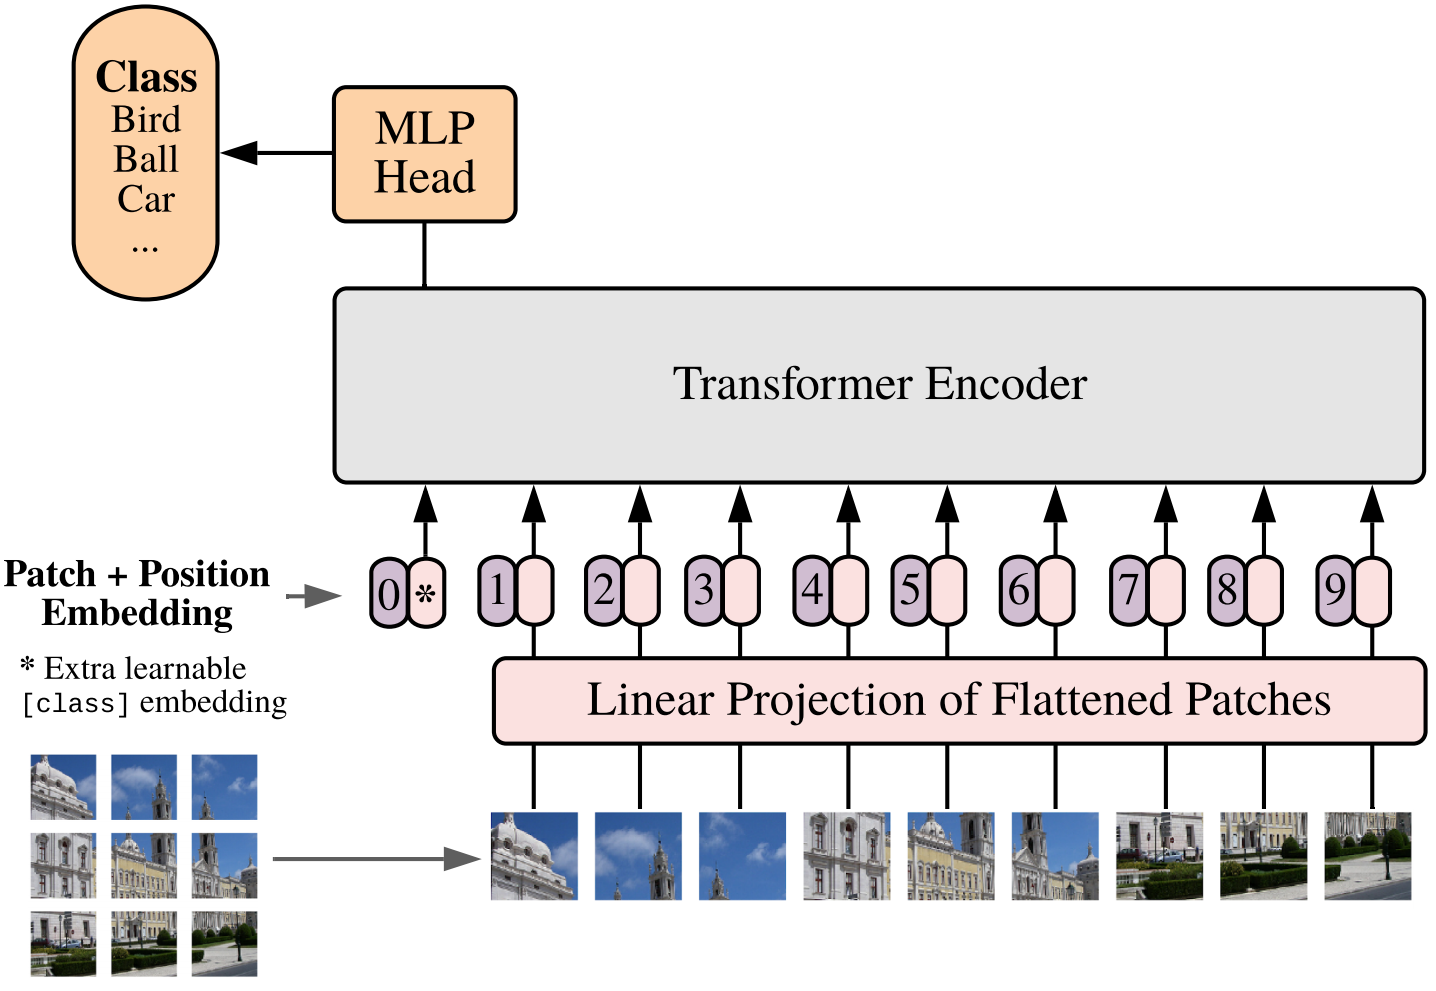
\includegraphics[width=.7\textwidth]{figure/vision-transformer.png}\\
	\beamergotobutton{\href{https://arxiv.org/abs/2010.11929}{Source: Dosovitskiy et al., 2020}}
\end{figure}

\begin{itemize}
	\item Split an image into fixed-size patches, treat each patch as a ``token'', and run an otherwise unmodified Transformer \textbf{encoder} over them.
	\item Encoder-only, exactly like BERT: a special classification token attends bidirectionally to every patch, and its final representation feeds a classification head -- ViT's {\tt [CLS]} token plays the same role BERT's does.
\end{itemize}

\vfill

\end{vbframe}

\begin{vbframe}{Transformer for multimodal learning}

\vfill

\textbf{CLIP}

\begin{figure}
	\centering
		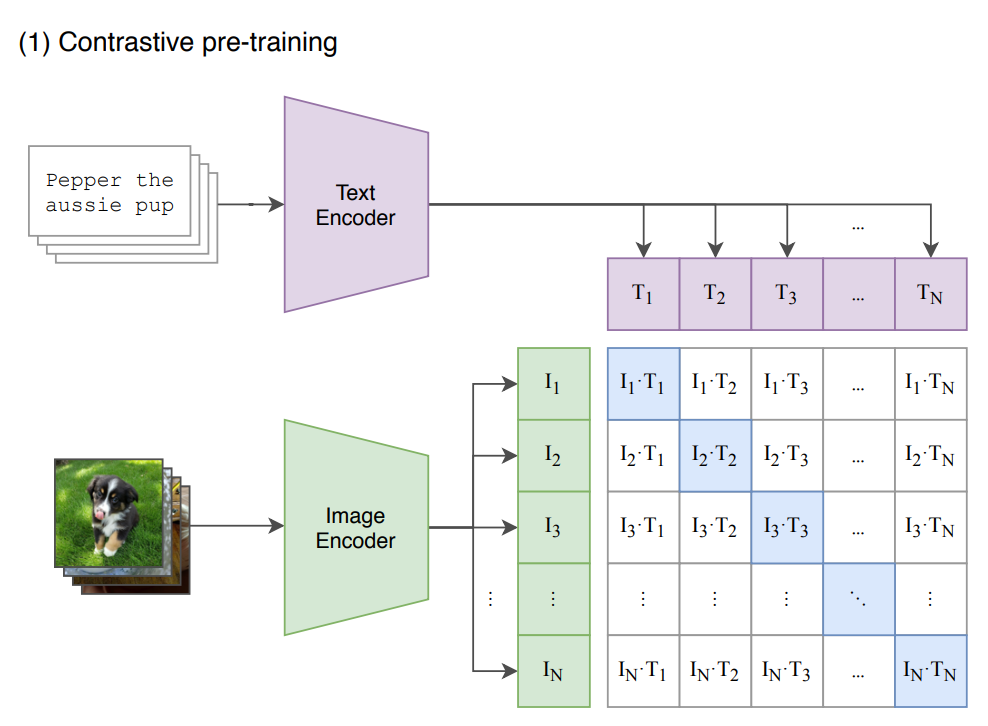
\includegraphics[width=.7\textwidth]{figure/clip1.png}\\
	\beamergotobutton{\href{https://arxiv.org/abs/2103.00020}{Source: Radford et al., 2021}}
\end{figure}

\vfill

\end{vbframe}

\begin{vbframe}{Transformer for multimodal learning}

\vfill

\textbf{CLIP}

\begin{figure}
	\centering
		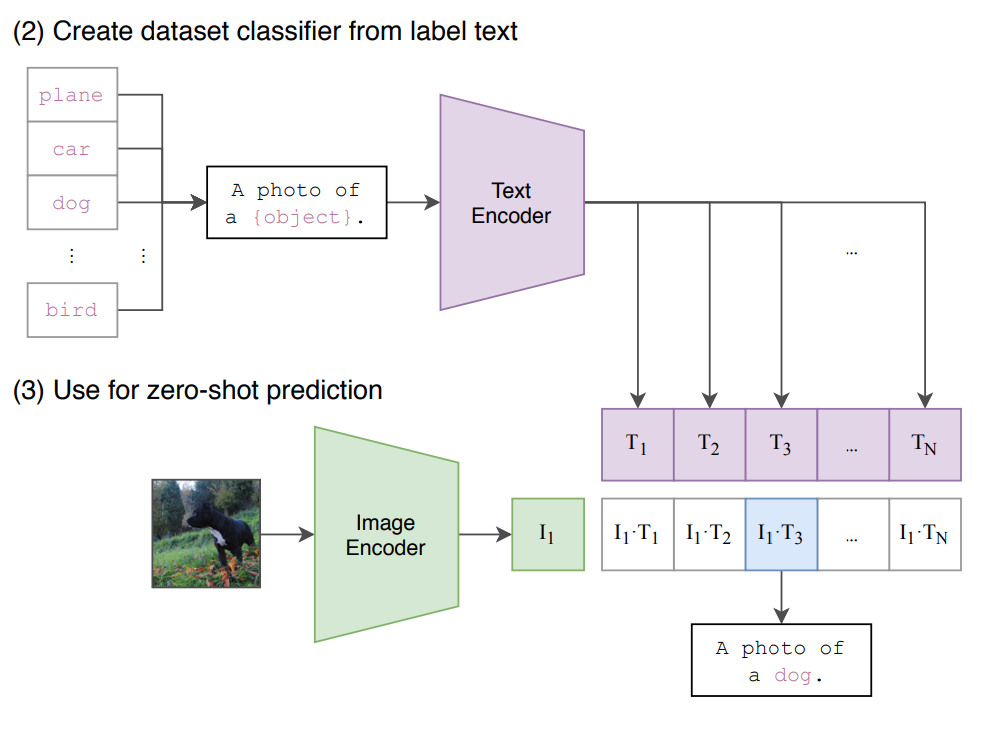
\includegraphics[width=.7\textwidth]{figure/clip2.png}\\
	\beamergotobutton{\href{https://arxiv.org/abs/2103.00020}{Source: Radford et al., 2021}}
\end{figure}

\vfill

\end{vbframe}

\begin{vbframe}{Transformer for multimodal learning}

\vfill

\textbf{FLAMINGO}

\begin{figure}
	\centering
		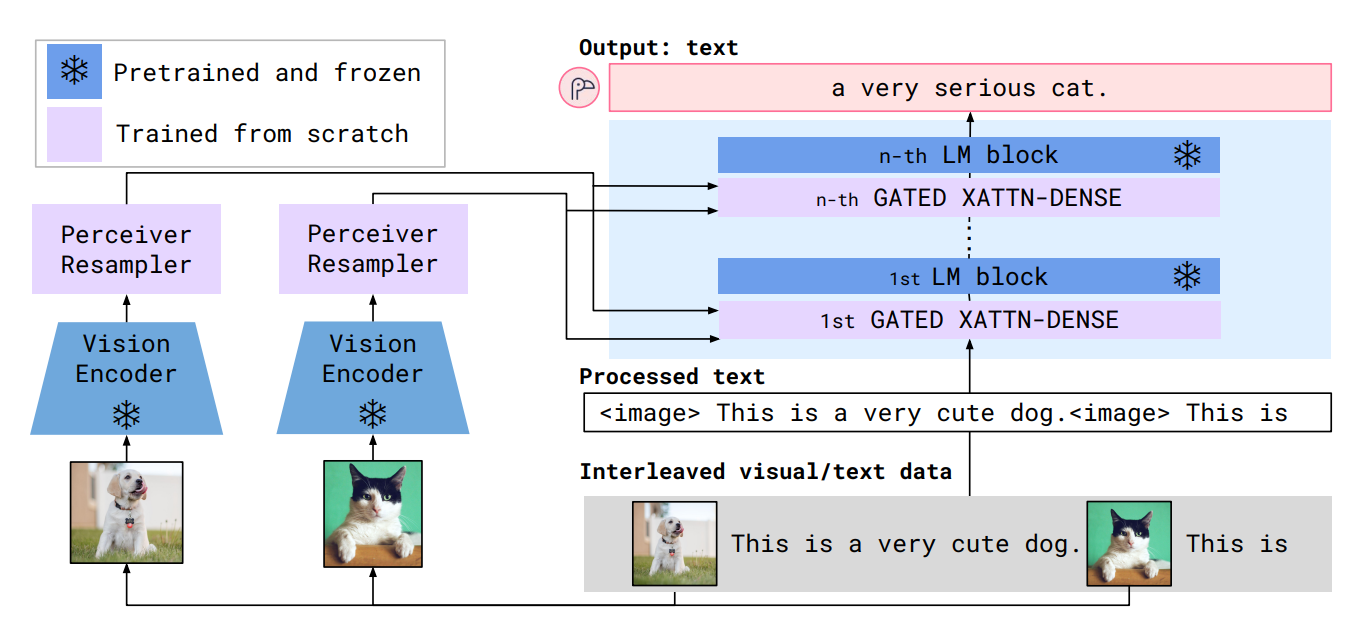
\includegraphics[width=.8\textwidth]{figure/flamingo.png}\\
	\beamergotobutton{\href{https://arxiv.org/pdf/2204.14198.pdf}{Source: Alayrac et al., 2022}}
\end{figure}

\vfill

\end{vbframe}

\begin{vbframe}{Transformer for multimodal learning}

\textbf{GPT-4}

\begin{figure}
	\centering
		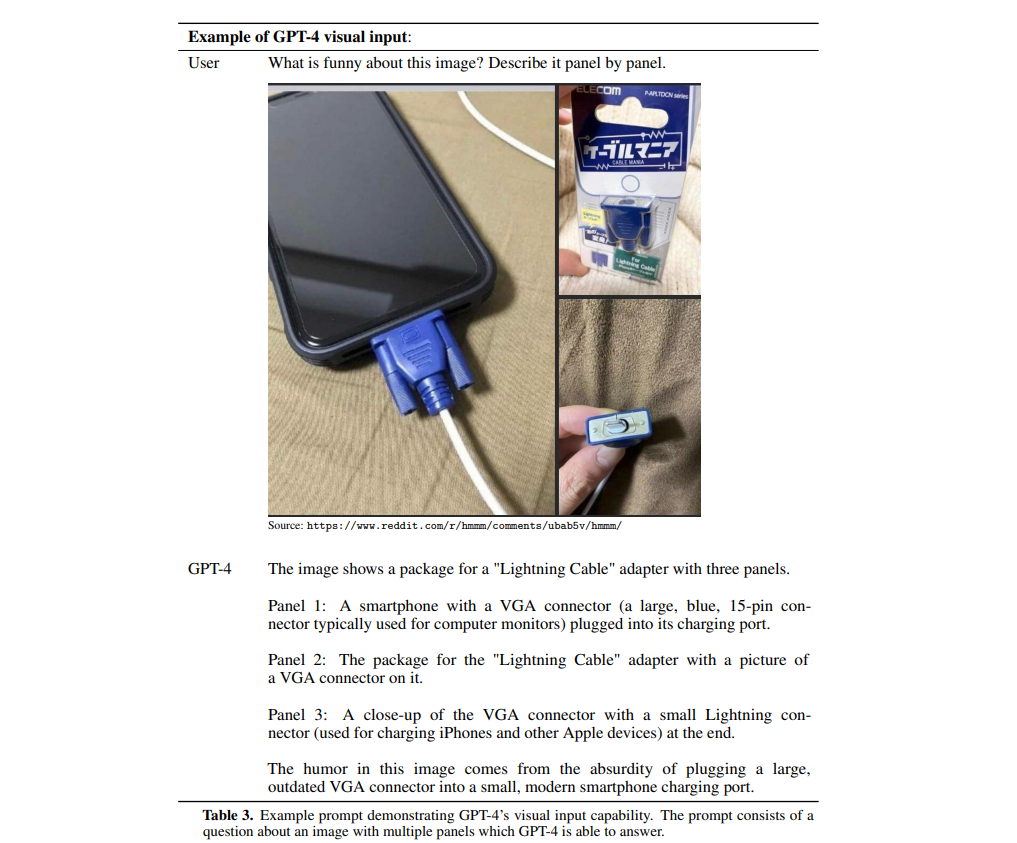
\includegraphics[width=.7\textwidth]{figure/gpt4.png}\\
	\beamergotobutton{\href{https://arxiv.org/pdf/2303.08774.pdf}{Source: OpenAI, 2023}}
\end{figure}

\end{vbframe}

%%%%%%%%%%%%%%%%%%%%%%%%%%%%%%%%%%%%%%%%%%%%%%%%%%%%%%%%%%%%%%%%%%

\section{BERT: Predecessors and Core Facts}
%%%%%%%%%%%%%%%%%%%%%%%%%%%%%%%%%%%%%%%%%%%%%%%%%%%%%%%%%%%%%%%%%%

\begin{vbframe}{Predecessors of BERT}

\begin{figure}
\centering
\includegraphics[width=10cm,page=5]{figure/transfer_learning_timeline1_nlp.pdf}
\end{figure}

\vfill

\textbf{Shortcomings of ELMo:}
\begin{itemize}
	\item No adaptation of the embeddings to the target domain/task; sequential LSTMs are not fully parallelizable.
\end{itemize}
\textbf{Alleviations, still each incomplete:}
\begin{itemize}
	\item ULMFiT \citebutton{Howard and Ruder, 2018}{https://www.aclweb.org/anthology/P18-1031}: a uni-directional LSTM fine-tuned as a whole model -- fine-tunable, but not bidirectional.
	\item GPT \citebutton{Radford et al., 2018}{https://s3-us-west-2.amazonaws.com/openai-assets/research-covers/language-unsupervised/language_understanding_paper.pdf}: a Transformer \textit{decoder}, fine-tuned as a whole model -- parallelizable and fine-tunable, but still not bidirectional.
\end{itemize}

\vfill

\end{vbframe}

\begin{vbframe}{BERT: Key Facts}

\vfill

\textit{\textbf{B}idirectional \textbf{E}ncoder \textbf{R}epresentations from \textbf{T}ransformers:}

\begin{itemize}
	\item Bidirectionally contextual: a token's embedding depends on both its left- and right-side context (like ELMo, but genuinely jointly, not two concatenated unidirectional passes).
	\item Completely replaces recurrence with self-attention $\to$ parallelizable, like GPT.
	\item The whole model can be fine-tuned, like GPT and ULMFiT.
	\item BERT is the first model to combine all three properties.
\end{itemize}

\framebreak

\begin{figure}
\centering
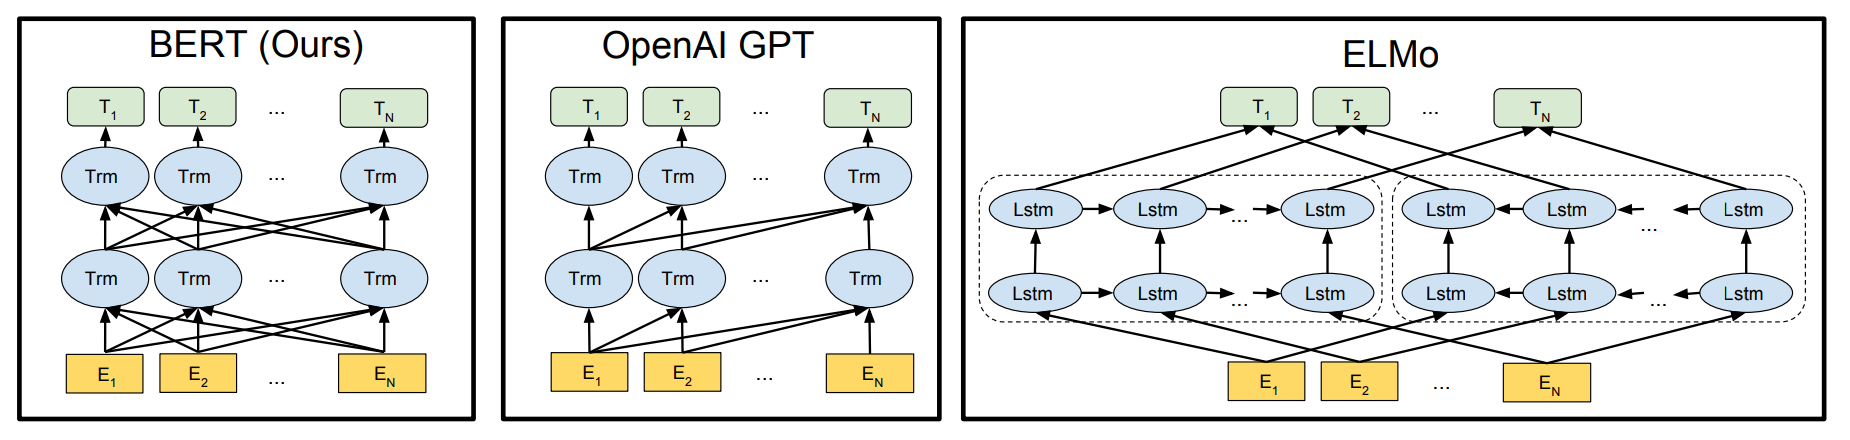
\includegraphics[width = 10cm]{figure/comparison-bert.png}\\
\citebutton{Source: Devlin et al., 2019}{https://aclanthology.org/N19-1423.pdf}
\end{figure}
$$Self\text{-}Attention + (Deep)\;Bidirectionality$$

\end{vbframe}

\begin{vbframe}{BERT: Architecture Numbers}

\vfill

\begin{itemize}
	\item Transformer \textit{encoder} as the entire backbone (the encoder from session 7, unmodified).
	\item Two sizes: 110M ($BERT_{Base}$) or 340M ($BERT_{Large}$) parameters.
	\begin{itemize}
		\item 12 (24) encoder blocks, embedding size $E = 768$ (1024), hidden size $H = E$, $A = H/64 = 12$ (16) attention heads, feed-forward size $4H$ -- exactly the shapes session 7's parameter-count derivation used variables for.
	\end{itemize}
\end{itemize}

\begin{figure}
	\centering
		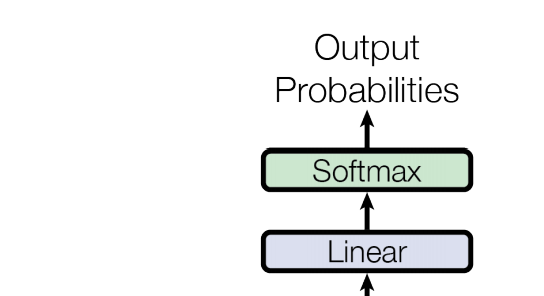
\includegraphics[width = 2.6cm]{figure/bert-top.png}\quad
		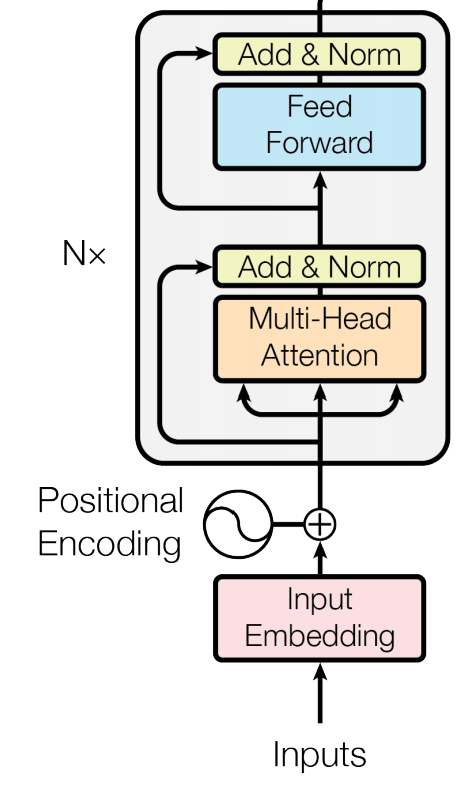
\includegraphics[width = 2.4cm]{figure/bert-bottom.png}\\
	\citebutton{Vaswani et al. (2017)}{https://arxiv.org/pdf/1706.03762.pdf}
\end{figure}

\vfill

\end{vbframe}

\begin{vbframe}{A Remark on Causality}

\vfill

\begin{itemize}
	\item \textbf{Self-supervision:} input and target sequence are the same, so the input must be modified to create a meaningful task.
	\item \warning Unconstrained (bidirectional) self-attention makes a language-modeling objective infeasible directly.
	\item \ques Why?
	\pause
	\item[] Bidirectionality would let a word see itself at a later hidden layer -- the model could ``cheat'' and would never learn a meaningful representation.
	\item This is exactly why BERT needs a \textit{different} training objective than plain next-token prediction -- covered next.
\end{itemize}

\vfill

\end{vbframe}

\begin{vbframe}{BERT -- Input and Output Embeddings}

\vfill

\begin{figure}
	\centering
	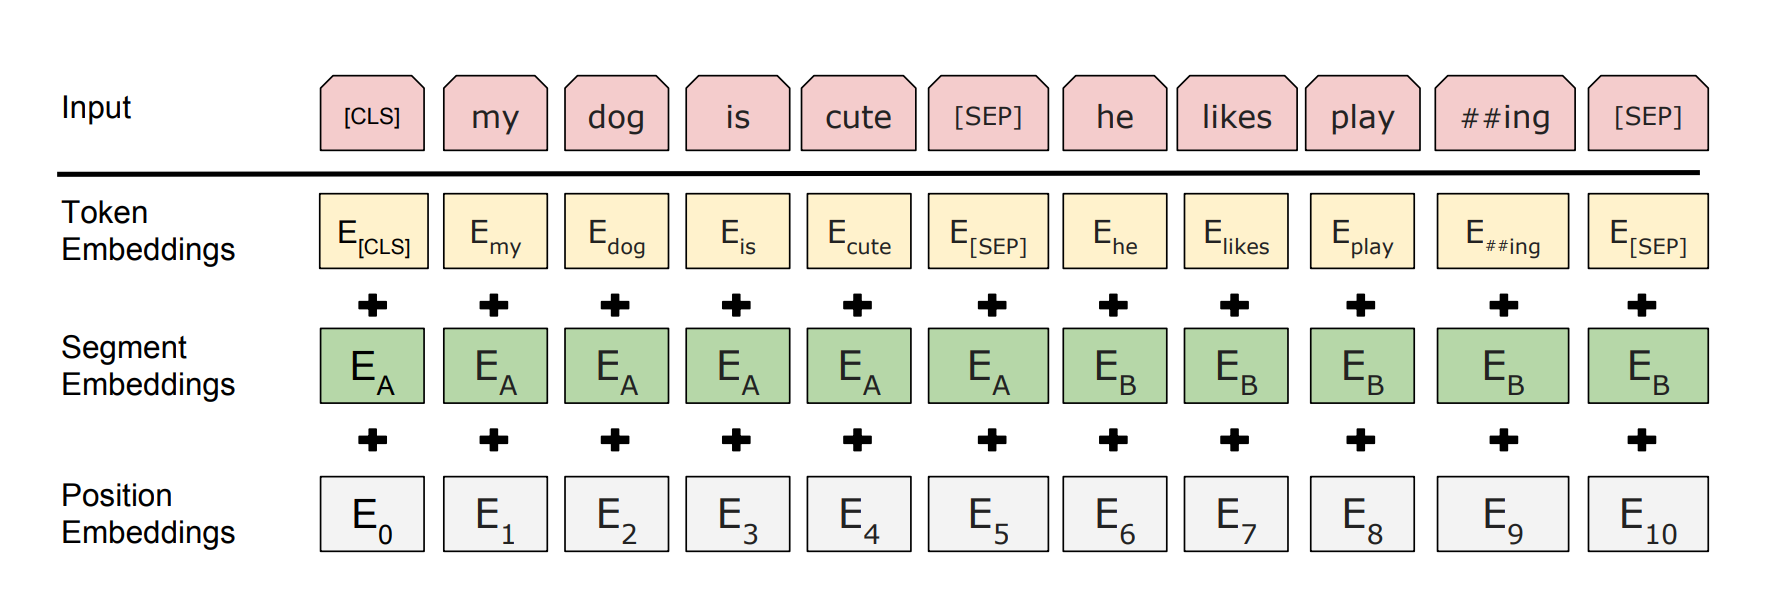
\includegraphics[width = 9cm]{figure/bert-input.png}\\
	\citebutton{Source: Devlin et al., 2019}{https://aclanthology.org/N19-1423.pdf}
\end{figure}

\begin{itemize}
	\item Two concatenated sentences as input, WordPiece-tokenized (Wu et al., 2016, session 7) into a 30,000-token vocabulary.
	\item \textit{Learned} segment and position embeddings (not sinusoidal, unlike the original Transformer).
	\item Special {\tt [CLS]} token: an overall sequence embedding, later used for classification. {\tt [SEP]}: separates the two sentences. {\tt [UNK]}: unknown tokens.
\end{itemize}

\framebreak

\begin{figure}
	\centering
	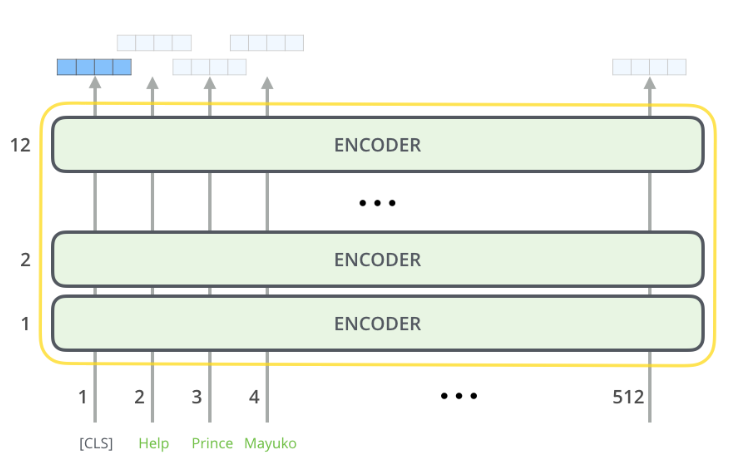
\includegraphics[width = 7cm]{figure/bert-embedings.png}\\
		\citebutton{Source: Jay Alammar}{https://jalammar.github.io/illustrated-bert/}
\end{figure}
Non-contextual at the input layer; more contextualized deeper into the stack -- one embedding per token, per layer.

\end{vbframe}

\begin{vbframe}{BERT Parameter Count}

\textit{From session 7 we already know one encoder layer costs $12\cdot d_{model}^2$ parameters:}
$$N_{Encoder} = n_{layers} \cdot 12\cdot d_{model}^2$$
\begin{itemize}
	\item \textbf{Base}: $12\cdot 12\cdot 768^2 = 84{,}934{,}656$
	\item \textbf{Large}: $24\cdot 12\cdot 1024^2 = 301{,}989{,}888$
\end{itemize}

\framebreak

\textit{Embeddings: let $V$ = vocabulary size, $M$ = max.\ sequence length, $S$ = number of segments -- all three are learned:}
$$N_{Embedding} = V\times d_{model} + S\times d_{model} + M\times d_{model}$$
With $V=30{,}000$, $S=2$, $M=512$:
\begin{itemize}
	\item \textbf{Base}: $30000\times768 + 2\times768 + 512\times768 = 23{,}434{,}752$
	\item \textbf{Large}: $30000\times1024 + 2\times1024 + 512\times1024 = 31{,}246{,}336$
\end{itemize}
Summing both parts: \textbf{Base} $\approx 108M \approx 110M$; \textbf{Large} $\approx 333M \approx 340M$.

\end{vbframe}

%%%%%%%%%%%%%%%%%%%%%%%%%%%%%%%%%%%%%%%%%%%%%%%%%%%%%%%%%%%%%%%%%%

\section{Autoregressive vs.\ Masked Language Modeling}
%%%%%%%%%%%%%%%%%%%%%%%%%%%%%%%%%%%%%%%%%%%%%%%%%%%%%%%%%%%%%%%%%%

\begin{vbframe}{Two Ways to Train a Language Model}
\begin{itemize}
	\item \textbf{Auto-regressive LMs (ARLMs)}: context = previous words, predict the next word; repeat, extending the prompt with each prediction. This is what session 9's GPT family does.
	\item \textbf{Masked LMs (MLMs)}: context = surrounding words (both sides), predict the masked word. This is what BERT does, and the reason it needs the causality workaround from the previous frame.
\end{itemize}
\end{vbframe}

\begin{vbframe}{ARLM: Worked Example}

\begin{figure}
	\centering
	\includegraphics[width=10cm,page=13]{figure/arlm.pdf}
\end{figure}

\begin{itemize}
	\item Starting from {\tt <START>}, the model outputs a probability distribution over the vocabulary at every step, picks a word (here, greedily), and feeds it back in as the next step's context -- one word at a time until the full sentence is built.
	\item Probabilistic interpretation, via the chain rule: $P(w_1,\ldots,w_n|w_0) = P(w_1|w_0)\cdot P(w_2|w_0,w_1)\cdots P(w_n|w_0,\ldots,w_{n-1})$ -- a clean estimate of $P(\text{sentence})$.
	\item Beyond text generation, this same recipe drives neural machine translation and image captioning (predict the next word/caption token given what came before).
\end{itemize}

\end{vbframe}

\begin{vbframe}{MLM: Worked Example}

\begin{figure}
	\centering
	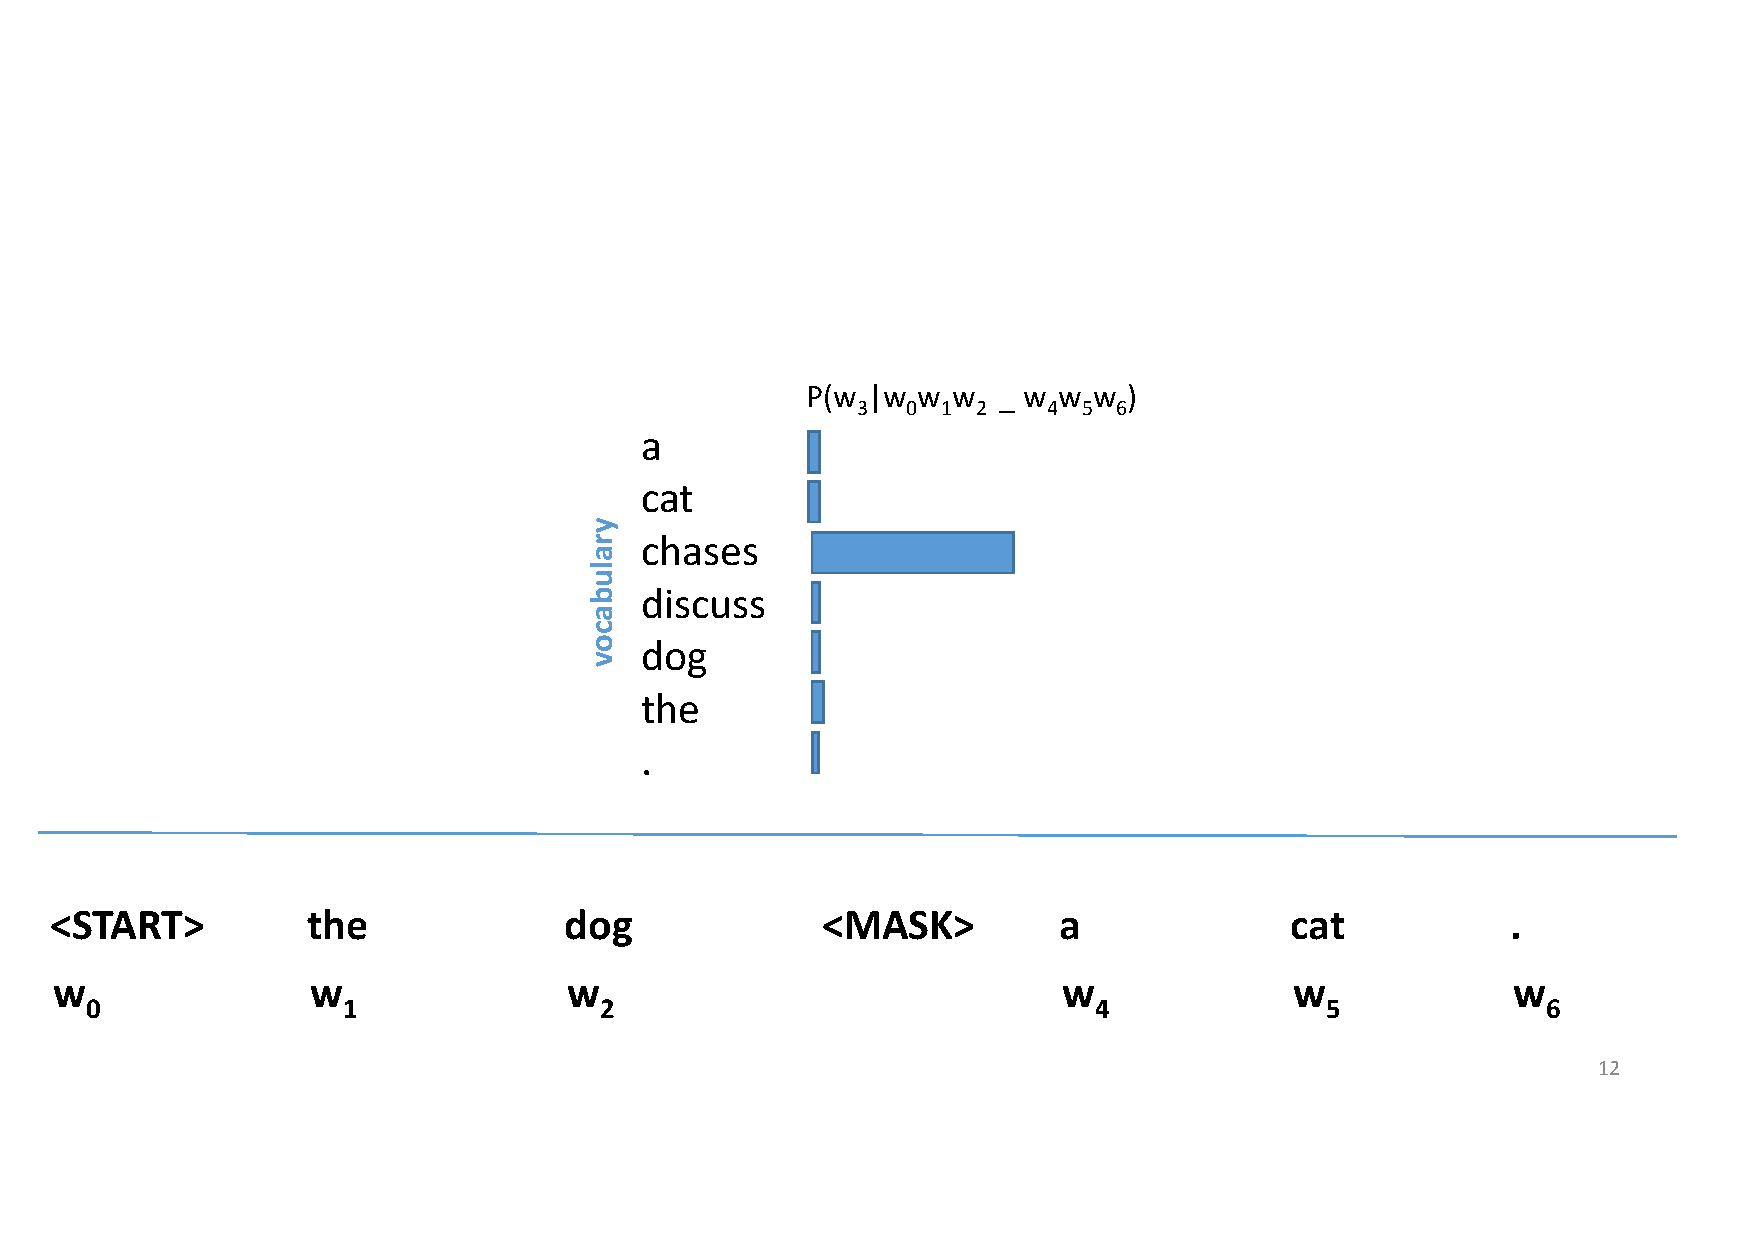
\includegraphics[width = 9cm]{figure/mlm.pdf}
\end{figure}

\begin{itemize}
	\item Estimates $P(w_i \mid w_0,\ldots,w_{i-1},w_{i+1},\ldots,w_n)$ for each masked position -- context from \emph{both} sides at once.
	\item No clean estimate of $P(\text{sentence})$ falls out of this (the per-token estimates don't chain-rule together the way ARLM's do) -- so ARLMs remain better for generation.
	\item MLM's advantage is exactly what it was designed for: learning contextualized \emph{representations}, not generating text.
\end{itemize}

\end{vbframe}

%%%%%%%%%%%%%%%%%%%%%%%%%%%%%%%%%%%%%%%%%%%%%%%%%%%%%%%%%%%%%%%%%%

\section{Pre-Training and Fine-Tuning BERT}
%%%%%%%%%%%%%%%%%%%%%%%%%%%%%%%%%%%%%%%%%%%%%%%%%%%%%%%%%%%%%%%%%%

\begin{vbframe}{Masked Language Modeling (MLM), Concretely}

\vfill

\begin{itemize}
	\item \textbf{Not} to be confused with masked \textit{self-attention} (the decoder's causal-masking mechanism, session 7) -- MLM is a training \textit{objective}, applied on top of ordinary (unmasked) self-attention.
	\item \textbf{Objective:} given a sentence, predict the {\tt [MASK]}ed tokens.
	\item \textbf{Sampling:} pick 15\% of tokens; of those, 80\% become {\tt [MASK]}, 10\% become a random token, 10\% are left unchanged.
\end{itemize}
\begin{center}
\footnotesize
\begin{tabular}{|cccccccccc|}
\hline
The & quick & brown & \cellcolor{blue!65}\texttt{[MASK]} & jumps & over & the & \cellcolor{blue!65}\texttt{[MASK]} & dog & . \\
\hline
\end{tabular}\\
Targets: (fox, lazy)
\end{center}

\framebreak

\begin{itemize}
	\item \warning Why not just always use {\tt [MASK]}? Because {\tt [MASK]} never occurs during fine-tuning -- pre-training with 100\%-{\tt [MASK]} would create a train/fine-tune mismatch.
	\item The 80/10/10 split ensures the model still has to build a real representation for \emph{every} selected position, whether or not it literally sees {\tt [MASK]} there.
\end{itemize}
\begin{figure}
	\centering
	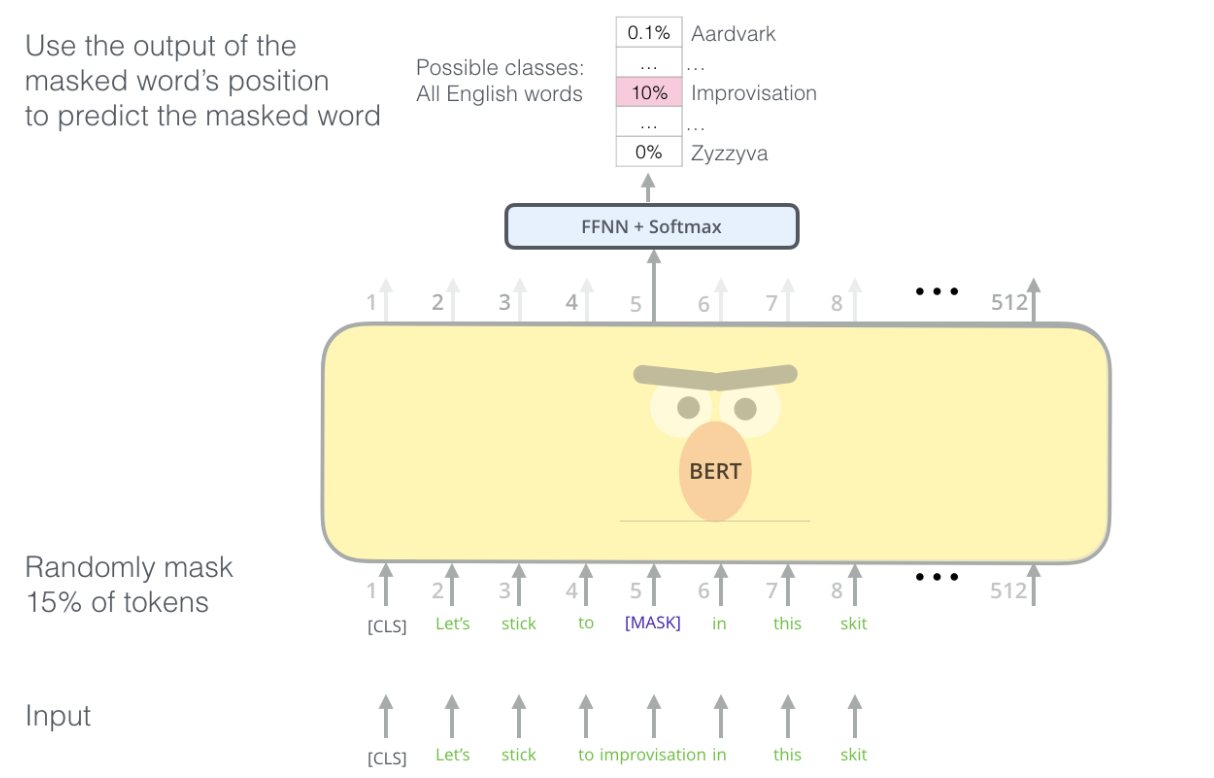
\includegraphics[width = 8cm]{figure/bert-mlm.png}\\
	\citebutton{Source: Jay Alammar}{https://jalammar.github.io/illustrated-bert/}
\end{figure}

\end{vbframe}

\begin{vbframe}{Next Sentence Prediction (NSP)}

\begin{itemize}
	\item \textbf{Objective:} given two sentences, predict whether the second follows the first (50\% real pairs, 50\% random).
	\item {\tt [CLS]}'s final representation feeds this (and later, any) sequence-level classification; {\tt [SEP]} marks the boundary.
\end{itemize}

\begin{figure}
	\centering
	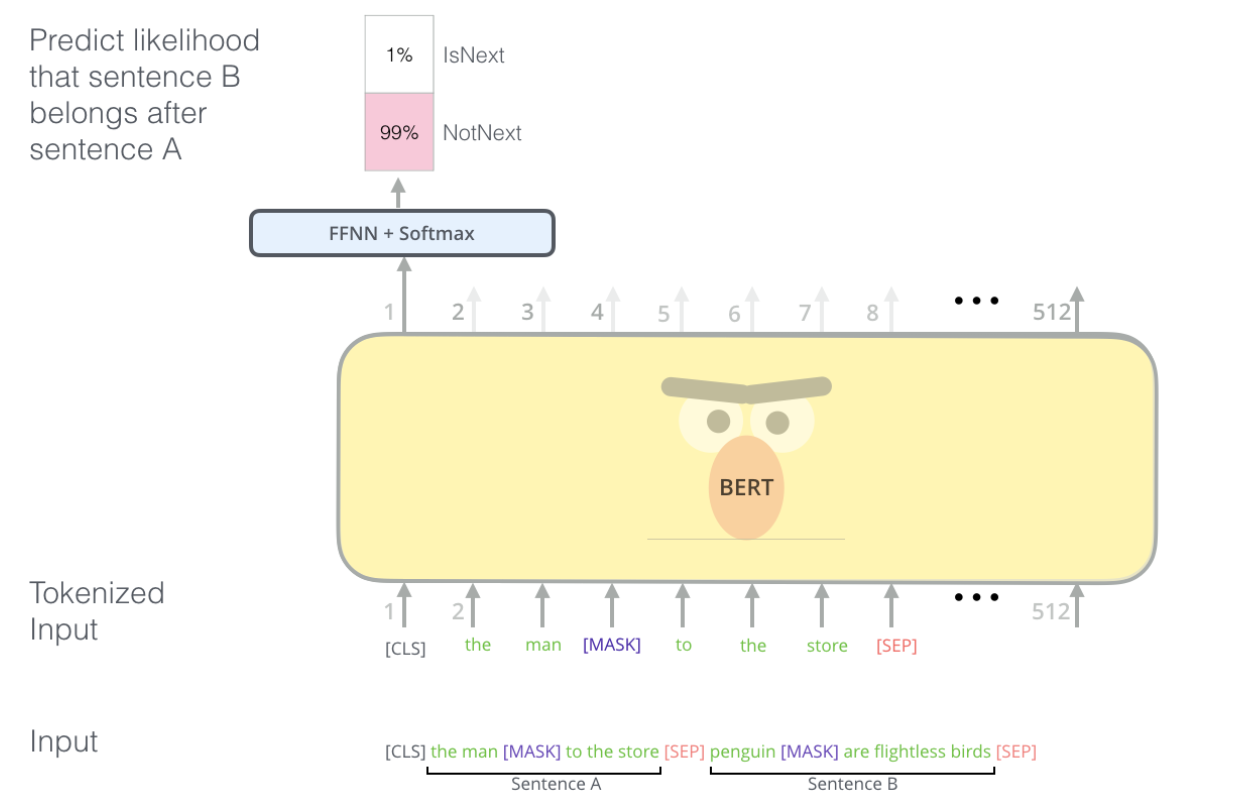
\includegraphics[width = 8cm]{figure/bert-nsp.png}\\
	\citebutton{Source: Jay Alammar}{https://jalammar.github.io/illustrated-bert/}
\end{figure}
$$Loss_{BERT} = Loss_{MLM} + Loss_{NSP}$$

\end{vbframe}

\begin{vbframe}{Pre-Training and Fine-Tuning}

\vfill

\textbf{Pre-training:} 13GB of text (BooksCorpus + English Wikipedia -- huge at the time, small by today's standards), $\sim$1M steps, batches of 256 sequences, mostly at sequence length 128 (10\% of steps at 512, since BERT's \emph{learned} position embeddings need long sequences to train well, but those are the expensive steps).

\framebreak

\begin{figure}
\centering
	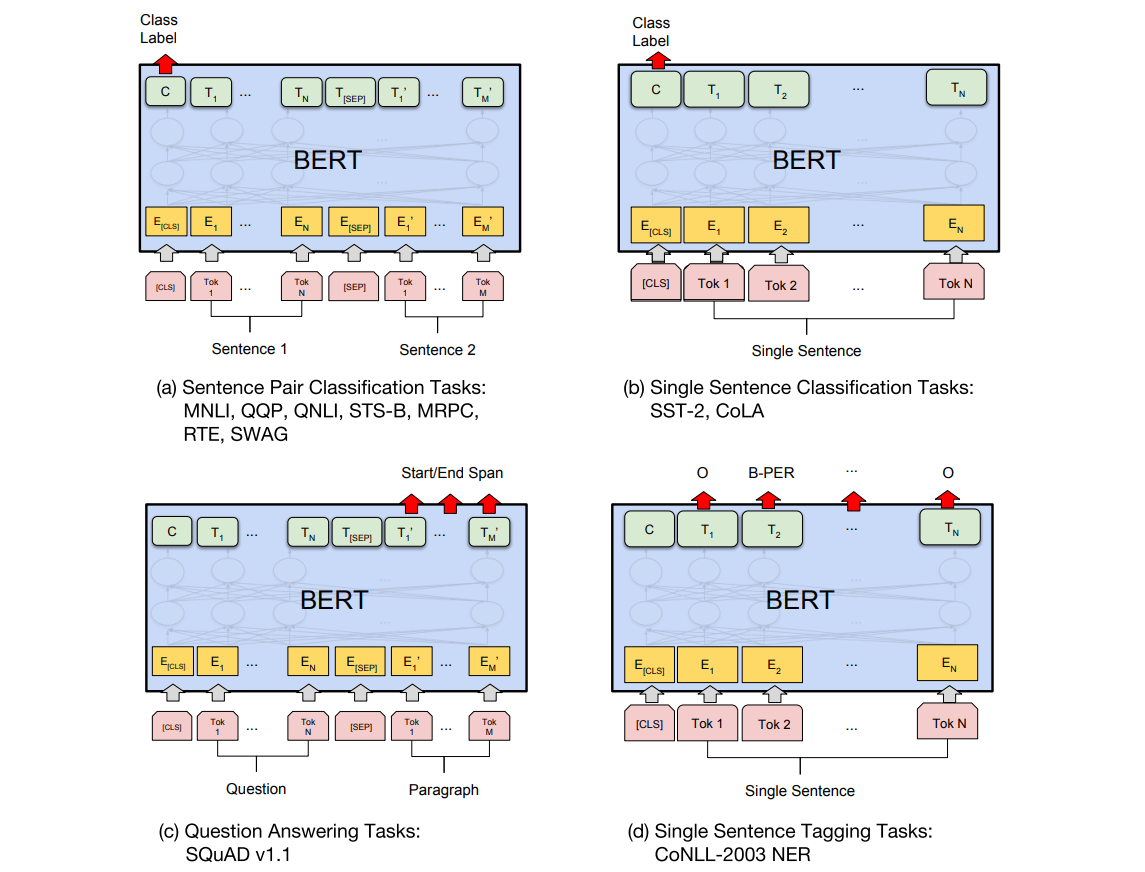
\includegraphics[width = 8cm]{figure/bert-finetune.png}\\
\citebutton{Source: Devlin et al., 2019}{https://aclanthology.org/N19-1423.pdf}
\end{figure}
\textbf{Fine-tuning:} cheap by comparison ($<$1h on a TPU, a few hours on a GPU); typical hyperparameters: batch size 16--32, learning rate 2--5e-5, 2--4 epochs. Beat every prior state-of-the-art on GLUE (Wang et al., 2018) at release -- since substantially surpassed by later models.

\end{vbframe}

\begin{vbframe}{Feature Extraction as an Alternative to Fine-Tuning}

\vfill

\begin{figure}
	\centering
	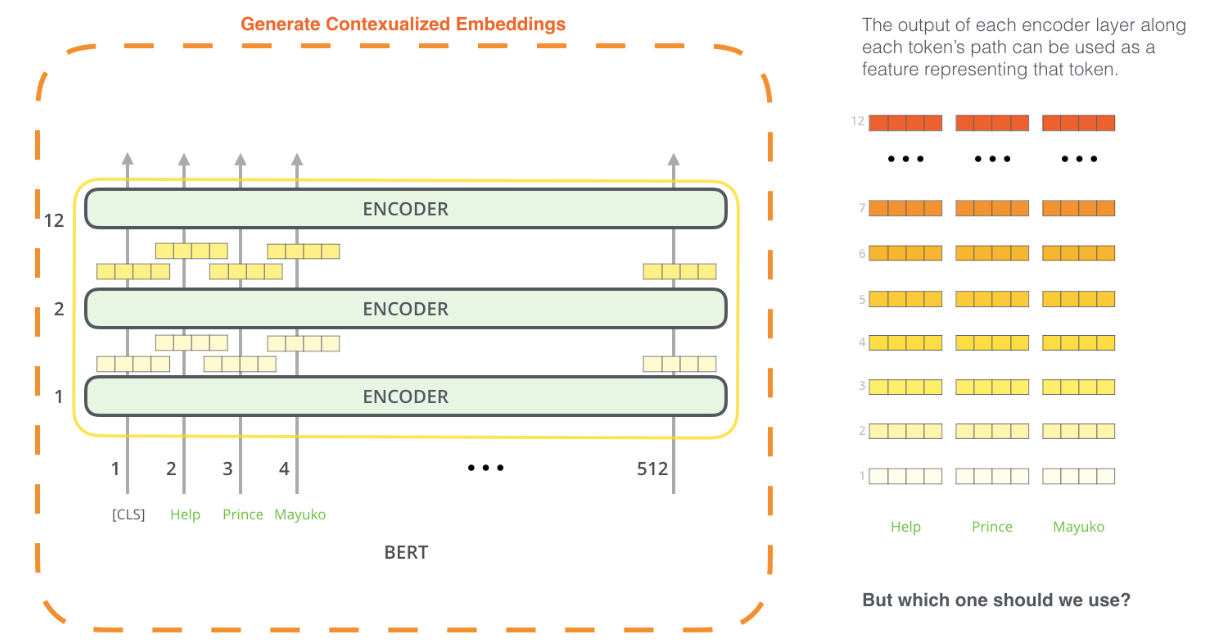
\includegraphics[width = 9cm]{figure/bert-featextr.png}\\
	\citebutton{Source: Jay Alammar}{https://jalammar.github.io/illustrated-bert/}
\end{figure}

\begin{itemize}
	\item Instead of fine-tuning BERT's own weights, freeze BERT and train only a small task-specific head on its output embeddings -- cheaper, at a small performance cost relative to full fine-tuning.
\end{itemize}

\vfill

\end{vbframe}

\begin{vbframe}{Measuring a Language Model: Perplexity}

\vfill

\begin{itemize}
	\item Well-defined for ARLMs (trickier for MLMs, for the same reason $P(\text{sentence})$ was): intuitively, how ``surprised'' the model is by a sequence.
	\item $$PPL = \exp\left(-\frac{1}{t}\sum_{i=1}^t \log p_\theta(w_i \mid w_{<i})\right)$$
	\item Lower bound 1 (perfect prediction); upper bound $|V|$ (uniform random guessing) -- a fair $k$-sided die has perplexity $k$.
\end{itemize}

\framebreak

\begin{itemize}
	\item \ques Is lower always better? Not necessarily comparable across corpora/languages/vocabulary sizes -- it's a useful \emph{relative} measure (no external labels needed), not an absolute one.
	\item Selection of reported values: 1B Word Benchmark ($|V|$=800k) PPL $\approx$ 21.8; WikiText-103 ($|V|$=270k) PPL $\approx$ 10.8; Penn Treebank ($|V|$=10k) PPL $\approx$ 20.5 -- note how much the vocabulary size alone affects what's achievable.
\end{itemize}

\vfill

\end{vbframe}

%%%%%%%%%%%%%%%%%%%%%%%%%%%%%%%%%%%%%%%%%%%%%%%%%%%%%%%%%%%%%%%%%%

\section{Self-Supervision and Transfer Learning}
%%%%%%%%%%%%%%%%%%%%%%%%%%%%%%%%%%%%%%%%%%%%%%%%%%%%%%%%%%%%%%%%%%

\begin{vbframe}{Feature-Based vs.\ Fine-Tuning Transfer}

\vfill

\textbf{Feature-based (e.g.\ word2vec, or frozen ELMo/BERT):} train an embedding model on a proxy task, then use its (frozen) output as features for a separate supervised model.

\textbf{Fine-tuning (e.g.\ BERT, GPT, ULMFiT):} pre-train the whole model, then continue training all (or most) of its own weights on the target task.

\vfill

\end{vbframe}

\begin{vbframe}{What Makes This ``Self-Supervised''?}

\vfill

\begin{itemize}
	\item \textbf{Unsupervised:} no labels; learn structure from features alone.
	\item \textbf{Supervised:} learn the association between (gold) labels and features.
	\item \textbf{Self-supervised:} no \emph{external} labels, but suitable labels can be generated automatically from the data's own structure (mask a word and use the original as the label) -- technically supervised learning, with none of the labeling cost and effectively unlimited training signal.
\end{itemize}

\vfill

\end{vbframe}

\begin{vbframe}{Self-Supervised Objectives, Beyond MLM}

\vfill

\begin{itemize}
	\item Skip-gram (word2vec), plain language modeling, and masked language modeling (BERT) are all self-supervised objectives -- differing only in which tokens are hidden from which context.
	\item \textbf{Permutation LM} (XLNet, Yang et al., 2019): autoregressive, but over a randomly permuted factorization order -- bidirectional context without ever introducing an artificial {\tt [MASK]} token. One sentence, because the mechanics (two attention ``streams'' to keep position and content separate) are a rabbit hole beyond this session's scope.
	\item \textbf{Replaced token detection} (ELECTRA, covered in full shortly): a second model has to tell real tokens from generated ones.
\end{itemize}

\vfill

\end{vbframe}

%%%%%%%%%%%%%%%%%%%%%%%%%%%%%%%%%%%%%%%%%%%%%%%%%%%%%%%%%%%%%%%%%%

\section{BERTology: What Does BERT Actually Learn?}
%%%%%%%%%%%%%%%%%%%%%%%%%%%%%%%%%%%%%%%%%%%%%%%%%%%%%%%%%%%%%%%%%%

\begin{vbframe}{Implications and Limitations}

\vfill

\begin{itemize}
	\item BERT changed how NLP research was done almost overnight -- probably as impactful as ChatGPT was in 2022, just without the general-public hype.
	\item That shift came with real limitations, several still open research questions today.
\end{itemize}

\vfill

\end{vbframe}

\begin{vbframe}{Limitation: Language Diversity}

\vfill

\begin{itemize}
	\item BERT was trained \emph{and evaluated} only on English (GLUE, SQuAD, RACE).
	\item Devlin et al.\ later released monolingual variants (varying in size, not language), then multilingual BERT (mBERT) for 100+ languages, giving a \emph{shared} embedding space across languages instead of needing to align separately-trained ones.
	\item This triggered a wave of language-specific BERTs: German, French (FlauBERT), Spanish (BETO), Dutch (BERTje), Chinese, Russian (RuBERT), Italian, and many more.
\end{itemize}

\vfill

\end{vbframe}

\begin{vbframe}{Limitation: Maximum Sequence Length}

\begin{figure}
\centering
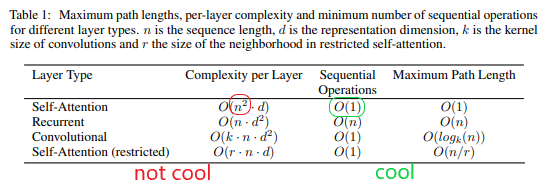
\includegraphics[width = 7cm]{figure/bert-problem.png}\\
	\beamergotobutton{\href{https://arxiv.org/abs/1706.03762}{Source: Vaswani et al., 2017}}
\end{figure}

\begin{itemize}
	\item BERT can only consume up to 512 tokens (the two NSP sentences together must fit this budget) -- the same $\mathcal{O}(n^2)$ self-attention cost from session 7's efficiency discussion, inherited unchanged.
\end{itemize}

\end{vbframe}

\begin{vbframe}{Limitation: Bias}

\vfill

\begin{itemize}
	\item Already known in static embeddings (\textit{``Man is to Computer Programmer as Woman is to Homemaker?''}, Bolukbasi et al., 2016) -- BERT learns whatever patterns exist in its training data, including social biases.
	\item StereoSet (Nadeem et al., 2021) measures this directly: a Stereotype Score (ideal $\approx$ 50, i.e.\ no stereotype preference) and a Language Model Score (ideal $\approx$ 100), combined into one ICAT score.
\end{itemize}

\begin{figure}
\centering
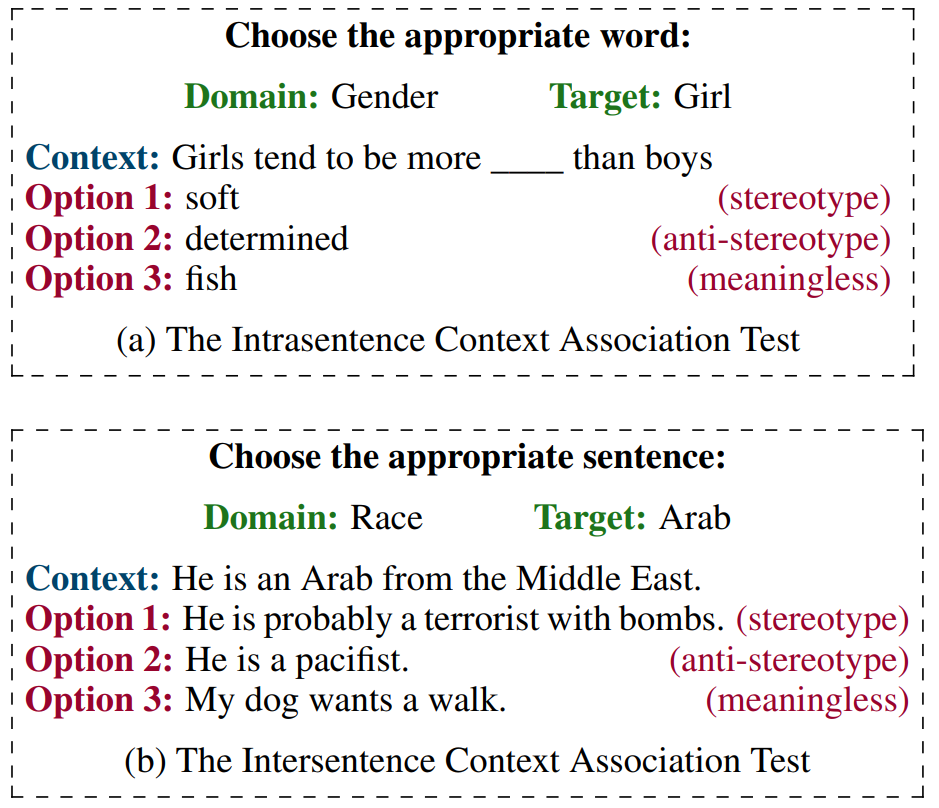
\includegraphics[width=6cm]{figure/stereoset.png}
\end{figure}

\vfill

\end{vbframe}

\begin{vbframe}{BERTology: Studying What's Inside}

\vfill

\begin{itemize}
	\item \textbf{BERTology} (Rogers et al., 2020; term coined by that survey): the field of study investigating the inner workings of large-scale Transformers like BERT -- does it encode syntactic/semantic/world knowledge, where is that knowledge localized, and how much of the architecture is actually necessary?
	\item Two influential findings: Clark et al.\ (2019) extracted BERT's attention maps over Wikipedia text and found interpretable patterns (attention concentrated on special tokens, on syntactic dependencies); Michel et al.\ (2019) found that at test time, most attention heads can be individually removed without hurting performance -- only $\sim$8 of 96 heads in their setup mattered.
	\item \warning Caveat: Jain and Wallace (2019) argue attention weights don't straightforwardly explain model behavior -- treat ``attention as explanation'' skeptically.
\end{itemize}

\vfill

\end{vbframe}

\begin{vbframe}{BERTology's Legacy: A Family of Follow-Ups}

\begin{figure}
	\centering
	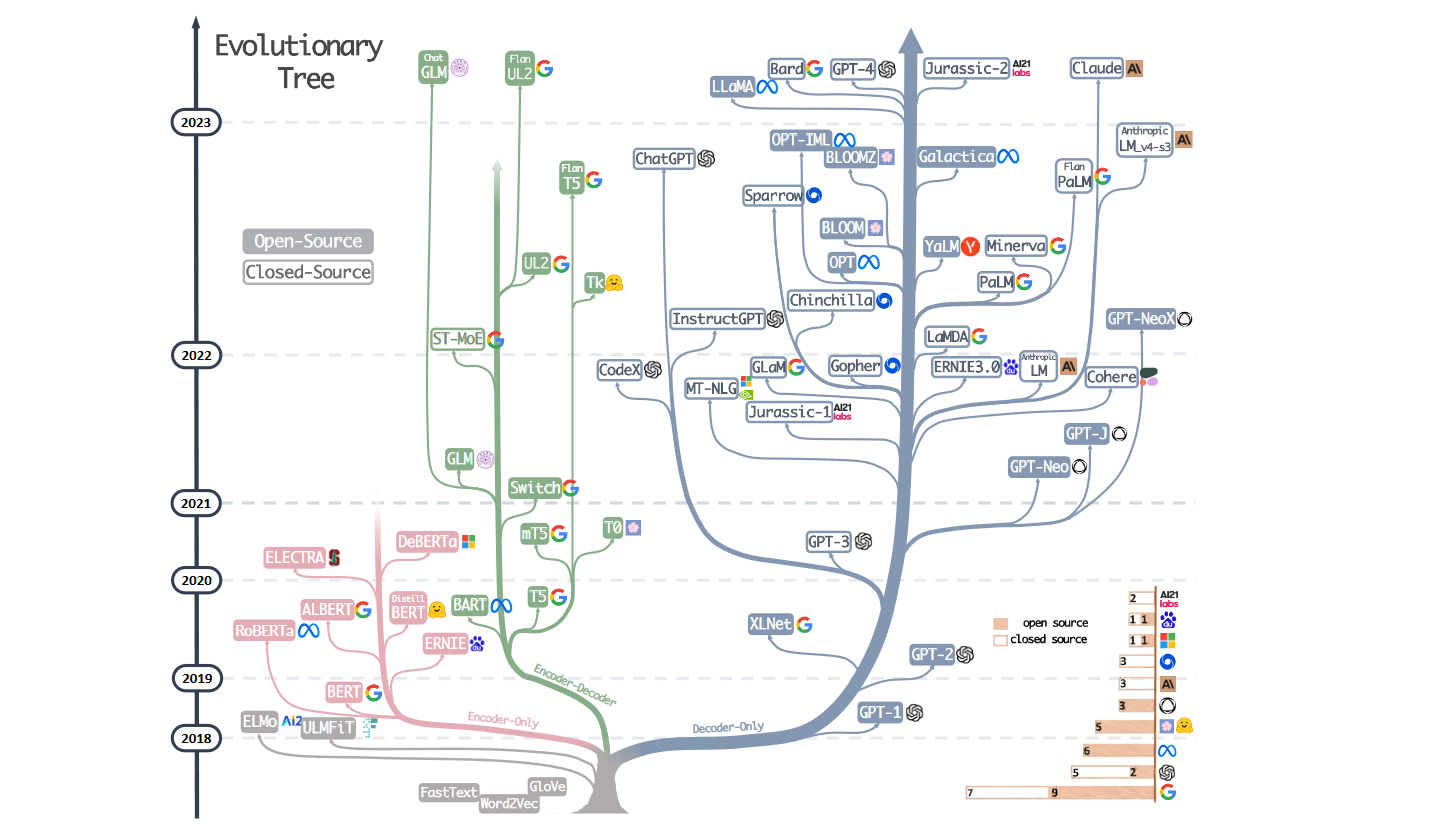
\includegraphics[width = 9cm]{figure/51-models.png}\\
	\citebutton{Source: Yang et al., 2023}{https://arxiv.org/abs/2304.13712}
\end{figure}

\begin{itemize}
	\item Almost every subsequent model still relies on the Transformer -- what changed is the pretraining objective, the parameter budget, or the architecture's efficiency. The rest of this session covers four representative directions: \textbf{better-trained} (RoBERTa), \textbf{parameter-efficient} (ALBERT), \textbf{distilled} (DistilBERT), and \textbf{differently-objectived} (ELECTRA).
\end{itemize}

\end{vbframe}

%%%%%%%%%%%%%%%%%%%%%%%%%%%%%%%%%%%%%%%%%%%%%%%%%%%%%%%%%%%%%%%%%%

\section{RoBERTa: A Better-Trained BERT}
%%%%%%%%%%%%%%%%%%%%%%%%%%%%%%%%%%%%%%%%%%%%%%%%%%%%%%%%%%%%%%%%%%

\begin{vbframe}{RoBERTa: Robustly Optimized BERT Approach}

\vfill

\citebutton{Liu et al., 2019}{https://arxiv.org/abs/1907.11692} -- same architecture as BERT, different \emph{training}:

\begin{itemize}
	\item \textbf{Dynamic masking}: BERT masks its corpus once, before training, so the same sequence is always masked the same way across all $\sim$40 epochs. RoBERTa duplicates the corpus and re-masks each copy differently, so the model sees each sequence masked in several distinct ways.
	\item \textbf{Drops NSP entirely} -- the authors found it hurt performance on several tasks.
	\item \textbf{More, longer training}: 160GB of text instead of 13GB, batches of 8k instead of 256, always at the full 512-token length. Their claim: BERT was simply \emph{undertrained}.
\end{itemize}

\framebreak

\begin{figure}
\centering
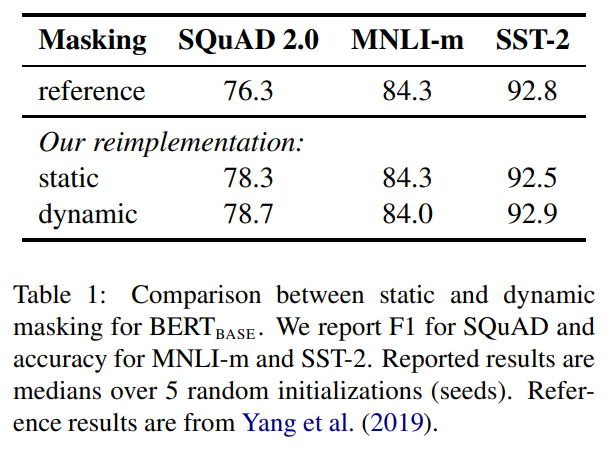
\includegraphics[width = 8cm]{figure/52-roberta-dynamic.png}\\
\citebutton{Source: Liu et al., 2019}{https://arxiv.org/abs/1907.11692}
\end{figure}
Same architecture, same parameter count class ($\sim$125M/360M, slightly larger due to a 50k-token BPE vocabulary vs.\ BERT's 30k) -- RoBERTa's gains come entirely from \emph{how} it was trained, not from any architectural change.

\end{vbframe}

%%%%%%%%%%%%%%%%%%%%%%%%%%%%%%%%%%%%%%%%%%%%%%%%%%%%%%%%%%%%%%%%%%

\section{ALBERT: A Parameter-Efficient BERT}
%%%%%%%%%%%%%%%%%%%%%%%%%%%%%%%%%%%%%%%%%%%%%%%%%%%%%%%%%%%%%%%%%%

\begin{vbframe}{ALBERT: A Lite BERT}

\vfill

\citebutton{Lan et al., 2019}{https://arxiv.org/abs/1909.11942} -- two architectural changes plus a new pretraining objective:

\begin{itemize}
	\item \textbf{Disentangle embedding size $E$ from hidden size $H$.} BERT ties $E=H$; ALBERT lets $H \gg E$: the (context-\emph{independent}) token embedding needs less capacity than the (context-\emph{dependent}) hidden representation, so growing $H$ without growing the $V\times E$ embedding matrix is far cheaper: $\mathcal{O}(V\times H) $ vs.\ $\mathcal{O}(V\times E + E\times H)$.
	\item \textbf{Cross-layer parameter sharing}: tie the attention and/or FFN weights across all layers -- a drastic size reduction, at some cost to performance (worse for sharing FFN than attention weights).
\end{itemize}

\framebreak

\begin{figure}
	\centering
	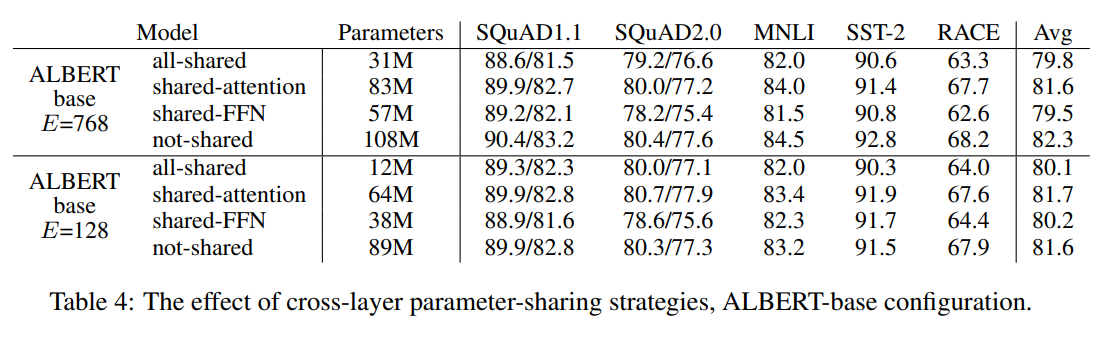
\includegraphics[width = 9cm]{figure/52-albert-param-sharing.png}\\
	\citebutton{Source: Lan et al., 2019}{https://arxiv.org/pdf/1909.11942.pdf}
\end{figure}

\begin{itemize}
	\item \textbf{Sentence-order prediction (SOP)} replaces NSP: same positive examples (two consecutive sentences), but negatives are the \emph{same two sentences swapped}, not a random sentence -- a harder, more useful signal than NSP's easy topic-mismatch shortcut.
	\item Result: much smaller models (except the scaled-up {\tt xxlarge} variant) at strong GLUE performance.
\end{itemize}

\end{vbframe}

%%%%%%%%%%%%%%%%%%%%%%%%%%%%%%%%%%%%%%%%%%%%%%%%%%%%%%%%%%%%%%%%%%

\section{DistilBERT: A Distilled BERT}
%%%%%%%%%%%%%%%%%%%%%%%%%%%%%%%%%%%%%%%%%%%%%%%%%%%%%%%%%%%%%%%%%%

\begin{vbframe}{Model Compression and Knowledge Distillation}

\vfill

\begin{itemize}
	\item \textbf{Motivation} \citebutton{Bucila et al., 2006}{http://www.niculescu-mizil.org/papers/rtpp364-bucila.rev2.pdf}: a large model generalizes well partly \emph{because} it's large (or an ensemble); can a small model be trained to mimic that behavior directly, rather than trained ``the normal way'' on labels alone?
	\item \textbf{Hard targets} $[0,0,0,1,0]$: ordinary one-hot labels. \textbf{Soft targets}: the teacher's own output distribution, optionally smoothed with a temperature $T$: $q_i = \exp(z_i/T) / \sum_j \exp(z_j/T)$ -- higher $T$ gives a softer distribution, carrying more information about which wrong answers the teacher considered plausible.
	\item Training the student on soft targets needs no ground-truth labels at all, and often a weighted mix of soft + hard targets works best.
\end{itemize}

\vfill

\end{vbframe}

\begin{vbframe}{DistilBERT}

\vfill

\begin{itemize}
	\item Student: half of BERT's layers (6 vs.\ 12 -- depth matters more for speed than hidden size), initialized directly from every other layer of a trained BERT; no segment embeddings (NSP is dropped, following RoBERTa).
	\item Three combined losses: distillation loss (soft targets), MLM loss (hard targets), and a cosine-embedding loss keeping DistilBERT's representations aligned with BERT's.
	\item Also adopts RoBERTa's dynamic masking and large-batch training.
\end{itemize}

\framebreak

\begin{figure}
	\centering
	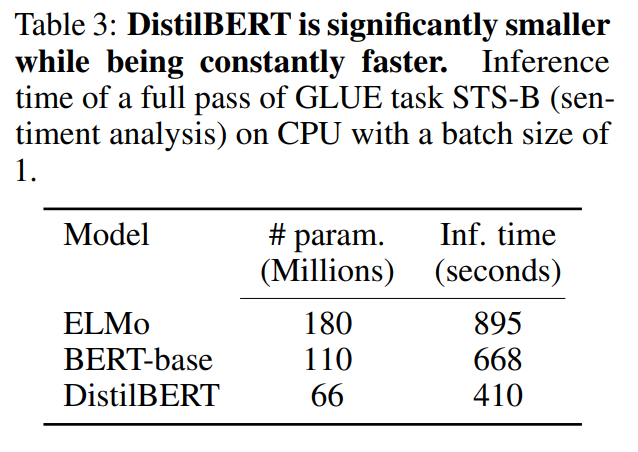
\includegraphics[width = 8cm]{figure/53-distilbert-size-speed.png}\\
	\citebutton{Source: Sanh et al., 2019}{https://arxiv.org/pdf/1910.01108.pdf}
\end{figure}

\begin{itemize}
	\item 40\% smaller, 60\% faster, retains $\sim$97\% of BERT's GLUE performance -- consistently a little behind BERT rather than better on any one task, which is exactly the expected trade for the size/speed win.
	\item Ablations: starting from BERT's own weights is the single biggest contributor; the cosine-embedding loss helps notably; dropping the MLM loss barely hurts (the soft-target signal alone is already strong).
\end{itemize}

\end{vbframe}

%%%%%%%%%%%%%%%%%%%%%%%%%%%%%%%%%%%%%%%%%%%%%%%%%%%%%%%%%%%%%%%%%%

\section{ELECTRA: A Different Pretraining Objective}
%%%%%%%%%%%%%%%%%%%%%%%%%%%%%%%%%%%%%%%%%%%%%%%%%%%%%%%%%%%%%%%%%%

\begin{vbframe}{ELECTRA: Replaced Token Detection}

\vfill

\citebutton{Clark et al., 2020}{https://arxiv.org/pdf/2003.10555.pdf} -- MLM's core inefficiency: only 15\% of tokens produce a learning signal per example. ELECTRA learns from \emph{all} of them.

\begin{itemize}
	\item Two Transformer encoders, trained jointly (not adversarially, despite superficially resembling a GAN): a small \textbf{generator} $G$ does ordinary MLM, replacing {\tt [MASK]}s with its own predictions; a large \textbf{discriminator} $D$ then sees the resulting corrupted sequence and predicts, \emph{for every token}, whether it's original or generator-produced.
\end{itemize}

\begin{figure}
	\centering
	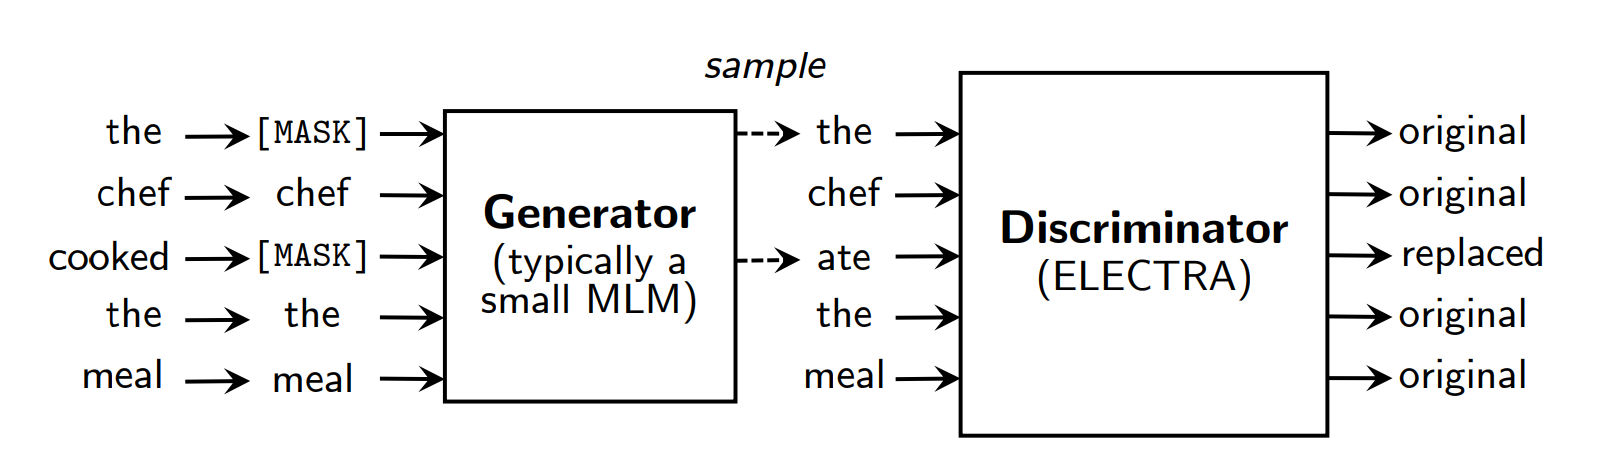
\includegraphics[width = 8cm]{figure/61-electra.png}\\
	\citebutton{Source: Clark et al, 2020}{https://arxiv.org/pdf/2003.10555.pdf}
\end{figure}

\framebreak

\begin{itemize}
	\item $G$: softmax over the vocabulary (as in MLM). $D$: per-token sigmoid, binary real-vs-generated.
	\item Combined loss weights $D$'s term $\times 50$, since it's typically much smaller than $G$'s.
	\item A \emph{smaller} generator (1/4--1/2 of $D$'s size) works best -- a generator as strong as $D$ makes the detection task too hard to learn from.
	\item At matched compute, ELECTRA beats RoBERTa and XLNet on GLUE; it was explicitly designed to be compute-efficient, not just accurate.
\end{itemize}

\end{vbframe}

%%%%%%%%%%%%%%%%%%%%%%%%%%%%%%%%%%%%%%%%%%%%%%%%%%%%%%%%%%%%%%%%%%

\section{From BERT to Text-to-Text}
%%%%%%%%%%%%%%%%%%%%%%%%%%%%%%%%%%%%%%%%%%%%%%%%%%%%%%%%%%%%%%%%%%

\begin{vbframe}{What's Still Missing?}

\vfill

BERT (and RoBERTa, ALBERT, DistilBERT, ELECTRA) all share the same recipe: pretrain an encoder, then attach a \emph{different, custom} classification head for each downstream task. Two problems follow directly from that:

\begin{itemize}
	\item \textbf{One fine-tuned copy per task} -- not realistic for many deployment scenarios (e.g.\ on-device), and the model never has a description of \emph{what task it's doing}; it just learns an association between text features and an arbitrary class-index vector like $[0,0,1,0,0,0]$.
	\item \textbf{Needs thousands of labeled examples per task} to fine-tune well, and risks overfitting to the idiosyncrasies of that particular labeled set -- very unlike how humans pick up a task from a description plus a handful of examples.
\end{itemize}

\vfill

\end{vbframe}

\begin{vbframe}{Idea: Describe the Task in Text, Too}

\vfill

\begin{itemize}
	\item If the model already takes text as input, why not prepend a natural-language \textbf{task description} to every example, instead of routing to a task-specific head?
	\item $$(\texttt{<task description>: <input>} \;;\; \texttt{<output as text>})$$
	\item Fine-tuned on enough such pairs, the model learns to associate the task description with the right output format -- and the exact wording of the description barely matters, as long as the model is fine-tuned on it (even a nonsense placeholder works, though a meaningful description that overlaps with pretraining data tends to help it learn faster).
	\item This immediately generalizes to \emph{multiple} tasks (each description routes to its own output space) and to \emph{generation}, not just classification: \texttt{translate English to German: ...}, \texttt{summarize: ...}, \texttt{predict sentiment: ...} \citebutton{Raffel et al., 2020}{https://jmlr.org/papers/v21/20-074.html}.
\end{itemize}

\vfill

\end{vbframe}

%%%%%%%%%%%%%%%%%%%%%%%%%%%%%%%%%%%%%%%%%%%%%%%%%%%%%%%%%%%%%%%%%%

\section{T5: Text-to-Text Transfer Transformer}
%%%%%%%%%%%%%%%%%%%%%%%%%%%%%%%%%%%%%%%%%%%%%%%%%%%%%%%%%%%%%%%%%%

\begin{vbframe}{T5: Every Task Is Text-to-Text}

\begin{figure}
	\centering
	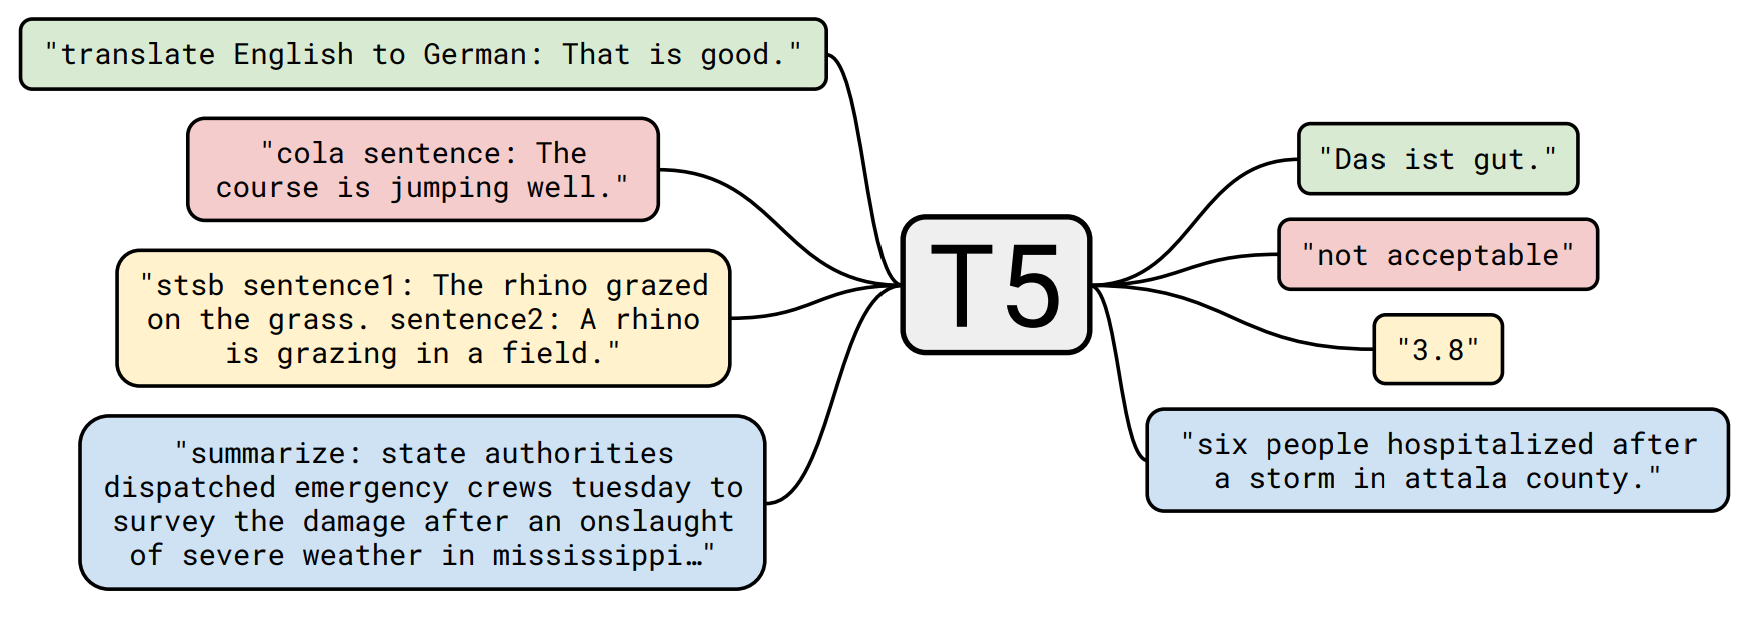
\includegraphics[width = 9cm]{figure/62-t5.png}\\
	\citebutton{Source: Raffel et al., 2020}{https://jmlr.org/papers/v21/20-074.html}
\end{figure}

\begin{itemize}
	\item A complete \textbf{encoder-decoder} Transformer (session 7's original architecture, not just an encoder like BERT) -- this session's flagship encoder-decoder example.
	\item Every task -- classification included -- is reframed as: input text (with a task prefix) in, output text out. Classification labels become words (e.g.\ \texttt{"positive"}), not indices.
	\item Sizes from 60M to 11B parameters; relative positional embeddings (Transformer-XL-style, session 7) rather than the original's sinusoidal or BERT's learned absolute ones.
\end{itemize}

\end{vbframe}

\begin{vbframe}{Why Not Just BERT's MLM Objective?}

\vfill

\begin{figure}
	\centering
	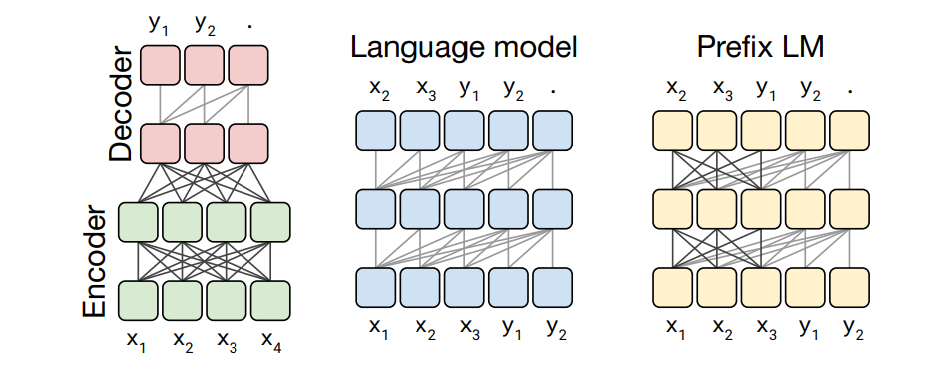
\includegraphics[width = 8cm]{figure/63-schematics.png}\\
	\citebutton{Source: Raffel et al., 2020}{https://jmlr.org/papers/v21/20-074.html}
\end{figure}

\begin{itemize}
	\item BERT's MLM predicts single masked tokens with a bidirectional encoder; T5's decoder is causal (it has to generate text), so its pretraining objective has to fit an encoder-decoder shape, not just an encoder.
\end{itemize}

\end{vbframe}

\begin{vbframe}{T5's Pretraining Objective: Span Corruption}

\begin{figure}
	\centering
	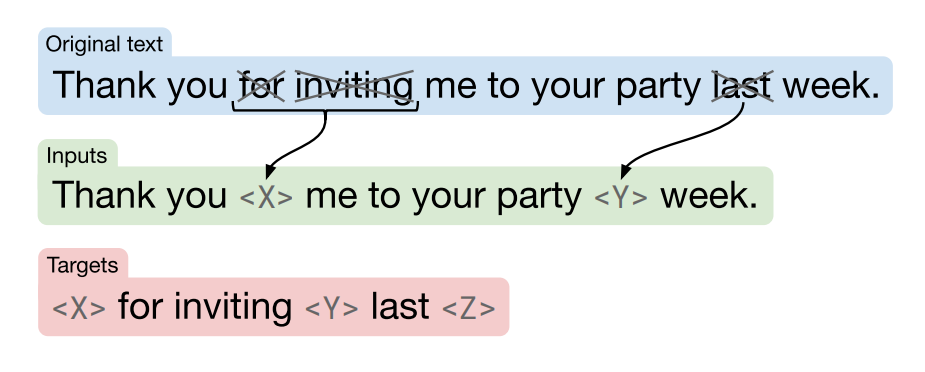
\includegraphics[width = 9cm]{figure/63-t5-span-pred.png}\\
	\citebutton{Source: Raffel et al., 2020}{https://jmlr.org/papers/v21/20-074.html}
\end{figure}

\begin{enumerate}
	\item Mark random \emph{spans} (not single tokens) in the input for corruption.
	\item Replace each corrupted span with a single sentinel token.
	\item The decoder's target: the sentinel tokens, each followed by the span it replaced.
\end{enumerate}
The encoder sees the corrupted input (bidirectionally); the decoder generates only the missing spans -- corrupting contiguous spans instead of scattered single tokens gave the best results among several objectives the authors tried, most of which were still MLM-flavored.

\end{vbframe}

\begin{vbframe}{Training Data and Scale: C4}

\vfill

\begin{itemize}
	\item \textbf{C4} (Colossal Clean Crawled Corpus): Common Crawl, filtered and cleaned for English -- 750GB, an order of magnitude larger than BERT's 13GB, built specifically to study how pretraining-data quality and size affect downstream performance.
	\item Exhaustive experiments across architecture (encoder-only vs.\ decoder-only vs.\ encoder-decoder), objective, model size (60M--11B), fine-tuning method, and multi-task mixing strategy.
	\item \textbf{Conclusions:} encoder-decoder wins for this text-to-text setting; more data and larger models both help, with larger-model-fewer-steps beating smaller-model-more-data; different denoising objectives perform similarly; fine-tuning \emph{all} parameters beats cheaper alternatives (adapters, partial unfreezing) when compute allows it. T5 beat BERT/RoBERTa-era models across GLUE, SuperGLUE, and translation benchmarks.
\end{itemize}

\vfill

\end{vbframe}

\begin{vbframe}{T5 Parameter Count}

\begin{center}
\footnotesize
\begin{tabular}{|c|c|c|c|}
\hline
\textbf{Model} & \textbf{Parameters} & $\bm{n_{layers}}$ & $\bm{d_{model}}$ \\ \hline
small  & 60M  & 6  & 512  \\ \hline
base   & 220M & 12 & 768  \\ \hline
large  & 770M & 24 & 1024 \\ \hline
\end{tabular}
\end{center}

\textit{Same recipe as session 7's Transformer parameter count, now with separate encoder and decoder terms and $V=32{,}000$:}
$$N_{Total} = n_{layers}\cdot(12\,d_{model}^2 + 16\,d_{model}^2) + 32000\times d_{model}$$
\begin{itemize}
	\item \textbf{Small}: $6\cdot 28\cdot 512^2 + 32000\times512 = 60{,}424{,}192$
	\item \textbf{Base}: $12\cdot 28\cdot 768^2 + 32000\times768 = 222{,}756{,}864$
	\item \textbf{Large}: $24\cdot 28\cdot 1024^2 + 32000\times1024 = 737{,}411{,}072$
\end{itemize}
{\footnotesize The 3B/11B variants break this formula -- they use $d_{FFN}\neq4d_{model}$ and $d_{qkv}\neq d_{model}/n_{heads}$, so their FFN/attention terms need to be re-derived individually; omitted here as a scaling detail beyond this session's scope.}

\end{vbframe}

%%%%%%%%%%%%%%%%%%%%%%%%%%%%%%%%%%%%%%%%%%%%%%%%%%%%%%%%%%%%%%%%%%

\section{Encoder-Decoder Beyond NLP: Whisper}
%%%%%%%%%%%%%%%%%%%%%%%%%%%%%%%%%%%%%%%%%%%%%%%%%%%%%%%%%%%%%%%%%%

\begin{vbframe}{Whisper: T5's Pattern, for Audio}

\vfill

\begin{itemize}
	\item \citebutton{Radford et al., 2022}{https://arxiv.org/abs/2212.04356}: the same encoder-decoder pattern as T5 and the original Transformer, with a spectrogram encoder in place of a text encoder.
	\item \textbf{Encoder}: bidirectional self-attention over a log-mel spectrogram of the audio (a spectrogram is itself just a 2D array of numbers -- no different in kind from the token embeddings T5's encoder consumes).
	\item \textbf{Decoder}: causal, cross-attends to the audio encoder's output, autoregressively generates transcript tokens -- for translation instead of transcription, only the decoder's target language changes.
	\item Confirms the taxonomy claim from the start of this session with a second, non-text example: the encoder-decoder pattern is about \emph{how information flows}, not about language at all.
\end{itemize}

\vfill

\end{vbframe}

%%%%%%%%%%%%%%%%%%%%%%%%%%%%%%%%%%%%%%%%%%%%%%%%%%%%%%%%%%%%%%%%%%

\section{Closing Synthesis}
%%%%%%%%%%%%%%%%%%%%%%%%%%%%%%%%%%%%%%%%%%%%%%%%%%%%%%%%%%%%%%%%%%

\begin{vbframe}{The Three Families, Revisited}

\begin{center}
\footnotesize
\begin{tabular}{@{}p{1.6cm}p{2.6cm}p{2.6cm}p{3.3cm}@{}}
\toprule
 & \textbf{Encoder-only} & \textbf{Decoder-only} & \textbf{Encoder-decoder} \\
\midrule
NLP & BERT, RoBERTa, ALBERT, DistilBERT, ELECTRA & GPT (session 9) & original Transformer, T5 \\[4pt]
Beyond NLP & Vision Transformer & autoregressive image/audio generation & Whisper (audio), Flamingo/GPT-4-style multimodal decoders \\
\bottomrule
\end{tabular}
\end{center}

\begin{itemize}
	\item Same architectural primitives throughout (self-attention, multi-head attention, positional encoding, residual connections, layer norm -- all from session 7); what changes across this whole table is only the attention pattern and the pretraining objective.
	\item Next up (session 9): decoder-only models, at scale -- GPT, and what actually changes once you make these models very large.
\end{itemize}

\end{vbframe}

%%%%%%%%%%%%%%%%%%%%%%%%%%%%%%%%%%%%%%%%%%%%%%%%%%%%%%%%%%%%%%%%%%
%%%%%%%%%%%%%%%%%%          REFERENCES          %%%%%%%%%%%%%%%%%%
%%%%%%%%%%%%%%%%%%%%%%%%%%%%%%%%%%%%%%%%%%%%%%%%%%%%%%%%%%%%%%%%%%
\begin{vbframe}
\frametitle{References}
\footnotesize{
\begin{thebibliography}{99}
\bibitem[(Devlin et al., 2019)]{bv1} Devlin, J., Chang, M.-W., Lee, K., \& Toutanova, K. (2019). \textit{BERT: Pre-training of Deep Bidirectional Transformers for Language Understanding}. \url{https://aclanthology.org/N19-1423/}
\bibitem[(Vaswani et al., 2017)]{bv2} Vaswani, A. et al.\ (2017). \textit{Attention Is All You Need}. \url{https://arxiv.org/abs/1706.03762}
\bibitem[(Howard \& Ruder, 2018)]{bv3} Howard, J., \& Ruder, S. (2018). \textit{Universal Language Model Fine-tuning for Text Classification}. \url{https://aclanthology.org/P18-1031/}
\bibitem[(Radford et al., 2018)]{bv4} Radford, A. et al.\ (2018). \textit{Improving Language Understanding by Generative Pre-Training}. OpenAI.
\bibitem[(Wu et al., 2016)]{bv5} Wu, Y. et al.\ (2016). \textit{Google's Neural Machine Translation System}. \url{https://arxiv.org/abs/1609.08144}
\bibitem[(Wang et al., 2018)]{bv6} Wang, A. et al.\ (2018). \textit{GLUE: A Multi-Task Benchmark and Analysis Platform for NLU}. \url{https://gluebenchmark.com/}
\bibitem[(Bolukbasi et al., 2016)]{bv7} Bolukbasi, T. et al.\ (2016). \textit{Man is to Computer Programmer as Woman is to Homemaker? Debiasing Word Embeddings}. \url{https://arxiv.org/abs/1607.06520}
\bibitem[(Nadeem et al., 2021)]{bv8} Nadeem, M., Bethke, A., \& Reddy, S. (2021). \textit{StereoSet: Measuring Stereotypical Bias in Pretrained Language Models}. \url{https://aclanthology.org/2021.acl-long.416/}
\bibitem[(Rogers et al., 2020)]{bv9} Rogers, A., Kovaleva, O., \& Rumshisky, A. (2020). \textit{A Primer in BERTology: What We Know About How BERT Works}. \url{https://aclanthology.org/2020.tacl-1.54/}
\bibitem[(Clark et al., 2019)]{bv10} Clark, K. et al.\ (2019). \textit{What Does BERT Look At? An Analysis of BERT's Attention}. \url{https://aclanthology.org/W19-4828/}
\bibitem[(Michel et al., 2019)]{bv11} Michel, P., Levy, O., \& Neubig, G. (2019). \textit{Are Sixteen Heads Really Better than One?} \url{https://arxiv.org/abs/1905.10650}
\bibitem[(Jain \& Wallace, 2019)]{bv12} Jain, S., \& Wallace, B. C. (2019). \textit{Attention is not Explanation}. \url{https://aclanthology.org/N19-1357/}
\bibitem[(Liu et al., 2019)]{bv13} Liu, Y. et al.\ (2019). \textit{RoBERTa: A Robustly Optimized BERT Pretraining Approach}. \url{https://arxiv.org/abs/1907.11692}
\bibitem[(Lan et al., 2019)]{bv14} Lan, Z. et al.\ (2019). \textit{ALBERT: A Lite BERT for Self-supervised Learning of Language Representations}. \url{https://arxiv.org/abs/1909.11942}
\bibitem[(Sanh et al., 2019)]{bv15} Sanh, V., Debut, L., Chaumond, J., \& Wolf, T. (2019). \textit{DistilBERT, a Distilled Version of BERT}. \url{https://arxiv.org/abs/1910.01108}
\bibitem[(Bucila et al., 2006)]{bv16} Bucil\u{a}, C., Caruana, R., \& Niculescu-Mizil, A. (2006). \textit{Model Compression}. KDD 2006.
\bibitem[(Hinton et al., 2015)]{bv17} Hinton, G., Vinyals, O., \& Dean, J. (2015). \textit{Distilling the Knowledge in a Neural Network}. \url{https://arxiv.org/abs/1503.02531}
\bibitem[(Clark et al., 2020)]{bv18} Clark, K. et al.\ (2020). \textit{ELECTRA: Pre-training Text Encoders as Discriminators Rather Than Generators}. \url{https://arxiv.org/abs/2003.10555}
\bibitem[(Yang et al., 2019)]{bv19} Yang, Z. et al.\ (2019). \textit{XLNet: Generalized Autoregressive Pretraining for Language Understanding}. \url{https://arxiv.org/abs/1906.08237}
\bibitem[(Raffel et al., 2020)]{bv20} Raffel, C. et al.\ (2020). \textit{Exploring the Limits of Transfer Learning with a Unified Text-to-Text Transformer}. \url{https://jmlr.org/papers/v21/20-074.html}
\bibitem[(Dosovitskiy et al., 2020)]{bv21} Dosovitskiy, A. et al.\ (2020). \textit{An Image is Worth 16x16 Words: Transformers for Image Recognition at Scale}. \url{https://arxiv.org/abs/2010.11929}
\bibitem[(Radford et al., 2021)]{bv22} Radford, A. et al.\ (2021). \textit{Learning Transferable Visual Models From Natural Language Supervision (CLIP)}. \url{https://arxiv.org/abs/2103.00020}
\bibitem[(Alayrac et al., 2022)]{bv23} Alayrac, J.-B. et al.\ (2022). \textit{Flamingo: a Visual Language Model for Few-Shot Learning}. \url{https://arxiv.org/abs/2204.14198}
\bibitem[(OpenAI, 2023)]{bv24} OpenAI (2023). \textit{GPT-4 Technical Report}. \url{https://arxiv.org/abs/2303.08774}
\bibitem[(Radford et al., 2022)]{bv25} Radford, A. et al.\ (2022). \textit{Robust Speech Recognition via Large-Scale Weak Supervision (Whisper)}. \url{https://arxiv.org/abs/2212.04356}
\end{thebibliography}
}
\end{vbframe}

%%%%%%%%%%%%%%%%%%%%%%%%%%%%%%%%%%%%%%%%%%%%%%%%%%%%%%%%%%%%%%%%%%
\section{License \& Attribution}
%%%%%%%%%%%%%%%%%%%%%%%%%%%%%%%%%%%%%%%%%%%%%%%%%%%%%%%%%%%%%%%%%%

\begin{vbframe}{License \& Attribution}
\begin{itemize}
\item The \enquote{Transformers Beyond NLP} section's five application frames (ViT, CLIP x2, Flamingo, GPT-4) were moved here from session 7's original \enquote{Transformer Motivation \& Applications} section (see that session's order.txt), to open this session with cross-domain evidence before the BERT/T5 deep dive.
\item All BERT, RoBERTa, ALBERT, DistilBERT, ELECTRA, and T5/text-to-text content is adapted from \textbf{Deep Learning for NLP (DL4NLP)}, SLDS, LMU Munich (chapters 4-6) --- licensed \textbf{CC BY 4.0}: \url{https://creativecommons.org/licenses/by/4.0/}. Condensed substantially from the source material (see order.txt for exactly what was cut and why), not reproduced in full.
\item The \enquote{Recap: The Three Transformer Families} section reuses (in adapted form) original text first written for session 7; the \enquote{Encoder-Decoder Beyond NLP: Whisper} frame and the \enquote{Closing Synthesis} table are original text written for this session, not adapted from any source.
\item Figures are used from their original DL4NLP sources; several (e.g.\ the BERT embeddings/MLM/NSP/feature-extraction illustrations) are themselves credited in DL4NLP's own slides to Jay Alammar's \textit{The Illustrated BERT} --- that attribution is preserved on each figure exactly as DL4NLP itself gives it, rather than re-attributed to DL4NLP.
\end{itemize}
\end{vbframe}

\endlecture
\end{document}
